\documentclass[11pt, a4paper]{article}

% --- PACOTES PRINCIPAIS ---
\usepackage[utf8]{inputenc}
\usepackage{geometry}
\geometry{a4paper, top=2.5cm, bottom=2.5cm, left=2.0cm, right=2.0cm}
\usepackage{amsmath, amssymb, amsfonts}
\usepackage{booktabs}
\usepackage{tabularx}
\usepackage{graphicx}
\usepackage{xcolor}
\usepackage{enumitem}
\usepackage{tcolorbox}
\usepackage{fancyhdr}
\usepackage{listings}
\usepackage{subcaption}
% --- CORES INSTITUCIONAIS UFOP ---
\definecolor{ufopred}{RGB}{140, 29, 36}
\definecolor{deepnavy}{RGB}{20, 35, 60}
\definecolor{lightgray}{RGB}{245, 247, 250}
\definecolor{darkslate}{RGB}{30, 40, 50}

% --- HYPERREF ---
\usepackage[
    colorlinks=true,
    linkcolor=ufopred,
    citecolor=deepnavy,
    urlcolor=ufopred
]{hyperref}


% --- ROTULOS EM PORTUGUES (o template nao carrega o babel) ---
\renewcommand{\figurename}{Figura}
\renewcommand{\tablename}{Tabela}

% --- CONFIGURAÇÃO DE CABEÇALHO E RODAPÉ ---
\pagestyle{fancy}
\fancyhf{}
\setlength{\headheight}{14pt}
\rhead{\textcolor{darkslate}{\small \textbf{BCC327 --- Computação Gráfica} --- TP1}}
\lhead{\textcolor{darkslate}{\small Árvores Arteriais CCO}}
\cfoot{\thepage}

\tcbuselibrary{skins, breakable}

% --- MARCADORES PARA O QUE O GRUPO PRECISA PREENCHER (buscar por "todo") ---
\newcommand{\todo}[1]{\textcolor{red}{\textbf{[#1]}}}
\newcommand{\figplaceholder}[3]{%
  \fcolorbox{red}{lightgray}{\parbox[c][#2][c]{#1}{\centering\color{red}\small #3}}}

% --- LISTAGENS DE CODIGO ---
\lstset{
  language=Python,
  basicstyle=\ttfamily\footnotesize,
  keywordstyle=\color{deepnavy}\bfseries,
  commentstyle=\color{gray}\itshape,
  backgroundcolor=\color{lightgray},
  frame=single, rulecolor=\color{deepnavy},
  breaklines=true, columns=fullflexible, aboveskip=6pt, belowskip=6pt
}

% --- CONTROLE DE ELEMENTOS FLUTUANTES ---
\usepackage{float}
\usepackage[section]{placeins}

\renewcommand{\topfraction}{0.85}
\renewcommand{\bottomfraction}{0.75}
\renewcommand{\textfraction}{0.10}
\renewcommand{\floatpagefraction}{0.80}

\setcounter{topnumber}{4}
\setcounter{bottomnumber}{3}
\setcounter{totalnumber}{5}
\begin{document}

% --- TÍTULO E AUTORES ---
\begin{center}
  {\LARGE \bfseries \textcolor{ufopred}{Visualização Geométrica, Rasterização e Recorte de Árvores Arteriais CCO: Uma Aplicação Didática de Computação Gráfica}}\\[0.4cm]

  {\large
    \textbf{\todo{Thiago Martins Zanete}}$^{1}$,
    \textbf{\todo{Gabriel Barony Menezes}}$^{1}$,
    \textbf{\todo{Samuel Braga Marques}}$^{1}$
  }\\[0.2cm]

  {\small
    $^{1}$Departamento de Computação (DECOM) --- Universidade Federal de Ouro Preto (UFOP)\\[0.1cm]
    \texttt{\{\todo{thiago.zanete}, \todo{gabriel.barony}, \todo{samuel.bm}\}@aluno.ufop.edu.br}
  }\\[0.2cm]

  {\small Trabalho Prático 1 --- BCC327 Computação Gráfica --- 2026.2}
\end{center}

\vspace{0.4cm}

% --- CAIXA DE RESUMO E PALAVRAS-CHAVE ---
\begin{tcolorbox}[colback=lightgray, colframe=deepnavy, arc=3pt, title=\textbf{RESUMO}, fonttitle=\bfseries]
\small
\textbf{Contexto:} Árvores arteriais sintéticas geradas pelo método \emph{Constrained Constructive Optimization} (CCO) são distribuídas como segmentos de reta em arquivos VTK, com o raio de cada vaso como atributo. Inspecionar esses modelos exige transformar dados geométricos em imagem, etapa que as bibliotecas gráficas costumam encapsular como uma caixa-preta.
\textbf{Objetivo:} Desenvolver uma aplicação que integre leitura, visualização, transformações geométricas, rasterização, antialiasing e recorte de árvores CCO, deixando explícito quais algoritmos clássicos foram implementados pelo grupo e quais foram delegados à biblioteca.
\textbf{Metodologia:} A aplicação foi escrita em Python com um leitor VTK próprio, PyVista para a janela 3D e para a câmera, e matrizes homogêneas $4\times4$ escritas pelo grupo. Os módulos didáticos (Bresenham, Scanline Fill, \emph{supersampling}, Cohen--Sutherland, Liang--Barsky e Sutherland--Hodgman) foram implementados sem funções de desenho ou de recorte de bibliotecas e conferidos automaticamente contra métodos independentes.
\textbf{Resultados:} Foram carregados quatro modelos 2D (8 a 256 terminais, 16 a 512 pontos). Os algoritmos concordaram com as referências em todos os testes: 202 polígonos para o Scanline, 40\,000 segmentos aleatórios para o recorte (com Cohen--Sutherland e Liang--Barsky idênticos) e 300 polígonos para o Sutherland--Hodgman. O \emph{supersampling} $4\times4$ reduziu o erro quadrático médio em relação a uma referência $16\times16$ de $4{,}68\times10^{-3}$ para $2{,}4\times10^{-4}$, cerca de 20 vezes.
\textbf{Conclusão:} O conjunto de módulos reproduz, com código próprio e verificável, as etapas de rasterização e recorte do \emph{pipeline} gráfico, e serve de base para os recursos de visibilidade, iluminação e textura previstos para o TP2.

\vspace{0.2cm}
\textbf{Palavras-Chave:} Computação Gráfica; Árvores Arteriais CCO; Rasterização; Antialiasing; Recorte de Segmentos e Polígonos.
\end{tcolorbox}

\vspace{0.4cm}

% --- SEÇÃO 1: INTRODUÇÃO E OBJETIVOS ---
\section{Introdução e Objetivos}
Modelos computacionais de redes vasculares são usados para estudar a perfusão de tecidos quando a resolução das imagens médicas não permite reconstruir a microcirculação. O algoritmo \emph{Constrained Constructive Optimization} (CCO), proposto por Schreiner e Buxbaum~\cite{schreiner1993}, gera árvores arteriais sintéticas de forma construtiva: segmentos terminais são inseridos um a um e a geometria de cada bifurcação é otimizada sob restrições. O resultado é uma árvore de segmentos retos, cada um com um raio associado.

Este trabalho trata da etapa seguinte: transformar esses dados geométricos em imagens. Não se implementa o método CCO, cujos modelos foram fornecidos pelo professor em formato VTK. O foco é a Computação Gráfica envolvida em visualizar a árvore, a saber, a escolha de primitivas e cores, as transformações e a câmera, a conversão de primitivas em pixels, a suavização de bordas e o recorte contra uma região de interesse.

Os objetivos do TP1 são: (i) ler e interpretar a estrutura dos modelos CCO; (ii) representá-los por linhas e tubos, com cor e espessura codificando o raio; (iii) aplicar translação, rotação e escala e controlar o observador; (iv) implementar os algoritmos de rasterização de linhas e polígonos; (v) comparar imagens com e sem antialiasing; (vi) implementar o recorte de segmentos e de polígonos; e (vii) documentar a divisão entre código próprio e código de biblioteca. As principais contribuições deste artigo são:
\begin{itemize}[leftmargin=*]
  \item um leitor de VTK legado ASCII escrito do zero, usado para explicar o formato e como alternativa ao PyVista;
  \item um visualizador interativo com transformações por matrizes homogêneas escritas pelo grupo e recorte interativo sobre o modelo;
  \item implementações próprias de Bresenham, Scanline Fill, \emph{supersampling}, Cohen--Sutherland, Liang--Barsky e Sutherland--Hodgman, cada uma com verificação automática contra um método independente;
  \item discussão comparativa de Cohen--Sutherland, Liang--Barsky e Cyrus--Beck, e de Sutherland--Hodgman e Weiler--Atherton.
\end{itemize}

% --- SEÇÃO 2: FUNDAMENTAÇÃO TEÓRICA ---
\section{Fundamentação Teórica}

\subsection{Árvores CCO e o formato VTK}
Os modelos fornecidos usam o formato VTK legado em ASCII, com \texttt{DATASET POLYDATA}. O arquivo contém uma seção \texttt{POINTS} (coordenadas $x,y,z$ de cada ponto), uma seção \texttt{LINES} (cada célula lista os índices dos pontos de um vaso) e uma seção \texttt{CELL\_DATA} com o escalar \texttt{raio}, um valor por segmento~\cite{schroeder2006}. Nos arquivos usados, cada célula é um segmento de dois pontos. Para uma árvore binária com $N$ terminais, há $2N$ pontos e $2N-1$ segmentos, e o segmento de índice 0 (a raiz) é o de maior raio. Todos os modelos fornecidos são planos ($z=0$).

\subsection{Transformações geométricas, mundo e câmera}
Um ponto $\mathbf{p}=(x,y,z)$ é representado em coordenadas homogêneas por $(x,y,z,1)^{T}$, de modo que translação, rotação e escala são todas multiplicações por matrizes $4\times4$:
\begin{equation}
  T(d_x,d_y,d_z)=\begin{pmatrix}1&0&0&d_x\\0&1&0&d_y\\0&0&1&d_z\\0&0&0&1\end{pmatrix},\quad
  S(s)=\begin{pmatrix}s&0&0&0\\0&s&0&0\\0&0&s&0\\0&0&0&1\end{pmatrix},\quad
  R_z(\theta)=\begin{pmatrix}\cos\theta&-\sin\theta&0&0\\\sin\theta&\cos\theta&0&0\\0&0&1&0\\0&0&0&1\end{pmatrix}.
  \label{eq:matrizes}
\end{equation}
As rotações $R_x$ e $R_y$ são análogas. Como a rotação e a escala atuam em torno da origem, para girar ou escalar o modelo em torno do seu centro $\mathbf{c}$ compõe-se
\begin{equation}
  M' = T(\mathbf{c})\,R\,T(-\mathbf{c})\,M,
  \label{eq:centro}
\end{equation}
em que $M$ é a transformação acumulada até o momento.

O \emph{espaço do mundo} é o sistema em que os vasos estão definidos (as coordenadas do arquivo, ajustadas pelas transformações do modelo). O \emph{sistema de coordenadas da câmera} tem origem no observador e eixos alinhados à sua orientação. A passagem de um para o outro é a matriz de visão: se o observador está em $\mathbf{e}$ e as colunas de $R_c$ são os eixos da câmera expressos no mundo, então $\mathbf{p}_c=R_c^{T}(\mathbf{p}_w-\mathbf{e})$. Mover o modelo e mover a câmera produzem imagens semelhantes, mas são operações distintas: a primeira altera as coordenadas no mundo, a segunda altera apenas a matriz de visão.

Na projeção \emph{ortográfica}, descarta-se a profundidade, $(x_s,y_s)=(x_c,y_c)$, e retas paralelas permanecem paralelas. Na projeção \emph{perspectiva}, com a câmera olhando ao longo de $+z_c$ e plano de projeção a uma distância $f$, tem-se $(x_s,y_s)=(f\,x_c/z_c,\;f\,y_c/z_c)$, e objetos mais distantes aparecem menores~\cite{hughes2013}.

\subsection{Rasterização de linhas e polígonos}
O algoritmo de Bresenham~\cite{bresenham1965} escolhe, a cada passo, o pixel mais próximo da reta ideal usando apenas somas e comparações de inteiros. Com $\Delta x=|x_1-x_0|$ e $\Delta y=|y_1-y_0|$, mantém-se um erro acumulado $e=\Delta x-\Delta y$ e decide-se avançar em $x$ se $2e>-\Delta y$ e em $y$ se $2e<\Delta x$; quando as duas condições valem, o passo é diagonal. O resultado tem exatamente $\max(\Delta x,\Delta y)+1$ pixels e funciona nos oito octantes.

O \emph{Scanline Fill} preenche um polígono varrendo as linhas horizontais da imagem. Para cada linha $y$, calculam-se os cruzamentos com as arestas, ordenam-se as abscissas e pintam-se os intervalos entre pares sucessivos (regra par-ímpar), o que trata corretamente polígonos côncavos~\cite{foley1990}.

\subsection{Aliasing e antialiasing}
Rasterizar equivale a amostrar uma imagem contínua em uma grade de pixels. Quando a imagem tem componentes de alta frequência espacial, como linhas inclinadas e contornos nítidos, a amostragem com uma única amostra por pixel produz serrilhado (\emph{aliasing}). O \emph{supersampling} (SSAA) amostra a cena $k\times k$ vezes por pixel e atribui ao pixel a média das amostras (filtro de caixa), de modo que pixels de borda recebem a cobertura parcial e tons intermediários. O MSAA, usado em GPUs, amostra a cobertura geométrica várias vezes por pixel, mas executa o cálculo de cor uma única vez, o que o torna mais barato que o SSAA.

\subsection{Recorte de segmentos e de polígonos}
\paragraph{Cohen--Sutherland.} Atribui a cada extremo um código de região de 4 bits (acima, abaixo, direita, esquerda) em relação à janela. Se os dois códigos são zero, o segmento é aceito; se o \emph{e} bit a bit dos códigos é diferente de zero, é rejeitado; nos demais casos, um extremo externo é movido até a borda indicada por um de seus bits e o teste se repete~\cite{newman1979}.

\paragraph{Liang--Barsky.} Escreve o segmento como $P(t)=P_0+t\,(P_1-P_0)$, $t\in[0,1]$, e impõe $p_k\,t\le q_k$ para cada borda $k$, com $(p_k,q_k)=(-\Delta x,\,x_0-x_{\min})$, $(\Delta x,\,x_{\max}-x_0)$, $(-\Delta y,\,y_0-y_{\min})$ e $(\Delta y,\,y_{\max}-y_0)$. Se $p_k<0$, o segmento \emph{entra} pela borda em $t=q_k/p_k$ e $t_0=\max(t_0,t)$; se $p_k>0$, \emph{sai} e $t_1=\min(t_1,t)$; se $p_k=0$ é paralelo, e é rejeitado quando $q_k<0$. Havendo $t_0>t_1$, nada é visível~\cite{liang1984}.

\paragraph{Cyrus--Beck.} É a base geral do Liang--Barsky: recorta contra qualquer janela \emph{convexa}, usando, para cada aresta, a normal externa $N_i$ e um ponto $P_i$ sobre ela. O cruzamento ocorre em $t=N_i\cdot(P_i-P_0)/(N_i\cdot d)$, e o sinal de $N_i\cdot d$ indica entrada ou saída~\cite{cyrus1978}. O Liang--Barsky é o caso particular da janela retangular alinhada aos eixos, em que as normais são $(\pm1,0)$ e $(0,\pm1)$ e os produtos escalares se reduzem à tabela de $p_k$ e $q_k$ acima. Neste trabalho, ele é apenas discutido.

\paragraph{Sutherland--Hodgman.} Recorta um polígono contra uma borda de cada vez, e a lista de vértices resultante de uma borda é a entrada da seguinte. Para cada aresta $s\to e$, aplicam-se quatro regras: ambos dentro, emite $e$; $s$ dentro e $e$ fora, emite a interseção; $s$ fora e $e$ dentro, emite a interseção e $e$; ambos fora, nada~\cite{sutherland1974}.

\paragraph{Weiler--Atherton.} Opera com duas listas circulares de vértices (polígono e janela) em que as interseções são inseridas e marcadas como entrada ou saída, e percorre os contornos alternando entre as listas. Produz um polígono por região resultante, o que o torna adequado a polígonos côncavos e a recortes com várias regiões ou furos~\cite{weiler1977}. Neste trabalho, ele é apenas discutido.

% --- SEÇÃO 3: METODOLOGIA E ARQUITETURA ---
\section{Metodologia e Arquitetura da Aplicação}

\subsection{Organização do código}
A aplicação é um conjunto coeso de módulos em Python: um visualizador interativo principal (\texttt{app.py}, que estende \texttt{visualizador.py}) e um conjunto de módulos didáticos independentes, executados por linha de comando, que geram as figuras e as verificações deste relatório. O visualizador usa o PyVista~\cite{sullivan2019}, uma interface em Python para o VTK, para a janela, a câmera e os tubos. Os módulos didáticos compartilham o leitor e o mapeamento mundo$\to$pixel de \texttt{util.py}. A Tabela~\ref{tab:arquivos} resume a organização.

\begin{table}[htbp]
  \centering
  \small
  \caption{Arquivos-fonte e módulos do TP1 que cada um atende.}
  \label{tab:arquivos}
  \begin{tabularx}{\textwidth}{l c X}
    \toprule
    \textbf{Arquivo} & \textbf{Módulo} & \textbf{Conteúdo} \\
    \midrule
    \texttt{readVtk.py} & 1 & Leitor próprio de VTK legado ASCII; resumo do modelo (pontos, segmentos, raios, limites, folhas) \\
    \texttt{visualizador.py} & 1, 2 & Visualizador PyVista: linhas e tubos, mapa de cores, matrizes de transformação, vistas e projeções \\
    \texttt{app.py} & 2, 6 & Aplicação principal: acrescenta rotação em $X$ e $Y$ e janela de recorte interativa \\
    \texttt{bresenham.py} & 3 & Bresenham, verificação e figuras \\
    \texttt{scanlineFill.py} & 4 & Scanline Fill, verificação, polígono dos extremos da árvore \\
    \texttt{antiAliasing.py} & 5 & \emph{Supersampling} sobre Bresenham e Scanline Fill, com erro quadrático médio \\
    \texttt{recorteSegmentos.py} & 6 & Cohen--Sutherland, Liang--Barsky, testes e comparação (Cyrus--Beck em comentário) \\
    \texttt{recorteArvore.py} & 6 & Recorte de todos os segmentos de uma árvore e figuras antes/depois \\
    \texttt{recortePoligonos.py} & 7 & Sutherland--Hodgman, testes e figuras (Weiler--Atherton em comentário) \\
    \texttt{util.py} & --- & Leitura via PyVista, mapeamento mundo$\to$pixel, raiz e folhas \\
    \bottomrule
  \end{tabularx}
\end{table}

\subsection{O que foi implementado pelo grupo e o que veio de bibliotecas}
A Tabela~\ref{tab:autoria} separa, funcionalidade por funcionalidade, o código próprio do que foi delegado a bibliotecas. O Matplotlib é usado apenas para exibir as grades e salvar as figuras, nunca para desenhar linhas, preencher polígonos ou recortar.

\begin{table}[htbp]
  \centering
  \small
  \caption{Autoria das funcionalidades: código do grupo $\times$ biblioteca.}
  \label{tab:autoria}
  \begin{tabularx}{\textwidth}{>{\raggedright\arraybackslash}p{4.3cm} >{\raggedright\arraybackslash}p{3.6cm} X}
    \toprule
    \textbf{Funcionalidade} & \textbf{Implementação} & \textbf{Observação} \\
    \midrule
    Leitura do VTK & Grupo e PyVista & \texttt{readVtk.py} é próprio; o visualizador e \texttt{util.py} usam \texttt{pv.read} \\
    Matrizes de translação, rotação e escala & Grupo & Matrizes $4\times4$ em NumPy aplicadas via \texttt{user\_matrix} do ator \\
    Janela, câmera, vistas e projeções & PyVista/VTK & \texttt{view\_xy}, \texttt{view\_xz}, \texttt{view\_yz}, \texttt{view\_isometric}, projeção paralela \\
    Tubos e mapa de cores & PyVista/VTK & Filtro \texttt{tube} e mapa \emph{viridis} \\
    Bresenham & Grupo & Sem funções de desenho de linha de biblioteca \\
    Scanline Fill & Grupo & Conferido com teste do raio \\
    \emph{Supersampling} & Grupo & Reutiliza Bresenham e Scanline Fill \\
    Cohen--Sutherland e Liang--Barsky & Grupo & Sem funções de recorte de biblioteca \\
    Sutherland--Hodgman & Grupo & Janela retangular alinhada aos eixos \\
    Cyrus--Beck e Weiler--Atherton & Apenas discussão & Seção~\ref{sec:discussao} \\
    \bottomrule
  \end{tabularx}
\end{table}

\subsection{Módulo 1 --- Leitura, primitivas e atributos}
O leitor próprio (\texttt{readVtk.py}) verifica o cabeçalho e o modo ASCII, separa o restante do arquivo em \emph{tokens} (de modo que a distribuição dos números em linhas não importa) e interpreta as palavras-chave \texttt{POINTS}, \texttt{LINES}, \texttt{CELL\_DATA}, \texttt{POINT\_DATA} e \texttt{SCALARS}. Uma célula com $k$ pontos vira $k-1$ segmentos consecutivos, os índices são validados e o atributo de raio é escolhido pelo nome (\texttt{raio} ou \texttt{radius}), com o primeiro escalar como alternativa. A função de resumo informa as grandezas pedidas no Módulo 1: dimensão (2D se todo $z$ é nulo), número de pontos e segmentos, raio mínimo e máximo e caixa envolvente.

O visualizador (\texttt{visualizador.py}) monta uma malha em que cada vaso tem seus próprios dois pontos. Isso é necessário porque um ponto compartilhado entre três vasos não poderia ter três raios ao mesmo tempo ao gerar os tubos. Há três modos de representação, alternados pela tecla \texttt{m}: (0) linhas coloridas pelo raio; (1) tubos com espessura e cor proporcionais ao raio; e (2) tubos apenas com espessura proporcional ao raio, em cor única. Como os raios do arquivo e as coordenadas estão em escalas diferentes, o raio visual é reescalado de modo que o vaso mais grosso tenha raio igual a 1,5\% da maior dimensão do modelo, e os demais mantêm a mesma proporção.

O modelo de cor adotado é um \emph{mapa contínuo} (\emph{viridis}) aplicado ao intervalo $[r_{\min},r_{\max}]$ do modelo carregado. Um mapa contínuo é preferível a canais RGB escolhidos à mão porque o raio é uma grandeza escalar e ordenada. O \emph{viridis} tem luminância monotônica e é perceptualmente uniforme, de modo que diferenças iguais de raio correspondem a diferenças visuais comparáveis, e permanece legível para pessoas com daltonismo~\cite{smith2015}. A barra de cores acompanha a imagem para permitir a leitura quantitativa.

\subsection{Módulo 2 --- Transformações e observador}
As matrizes da Equação~\ref{eq:matrizes} (e as de $R_x$ e $R_y$, em \texttt{app.py}) são funções do grupo. A transformação acumulada é mantida como uma única matriz $4\times4$ e atribuída ao ator do PyVista; cada comando do usuário multiplica essa matriz à esquerda, como na Equação~\ref{eq:centro}, de modo que a rotação e a escala ocorrem em torno do centro \emph{atual} do modelo. A translação usa um passo de 5\% da maior dimensão, a rotação usa $10^{\circ}$ e a escala usa o fator $1{,}1$ (ou $1/1{,}1$). O observador é controlado de duas formas: quatro vistas predefinidas (\texttt{xy}, \texttt{xz}, \texttt{yz} e isométrica), alternadas pela tecla \texttt{v}, e a câmera do PyVista, movida pelo mouse. A tecla \texttt{o} alterna entre projeção ortográfica (projeção paralela) e perspectiva. Os comandos estão na Tabela~\ref{tab:comandos}.

\begin{table}[htbp]
  \centering
  \small
  \caption{Comandos da aplicação principal (\texttt{app.py}).}
  \label{tab:comandos}
  \begin{tabularx}{\textwidth}{l X}
    \toprule
    \textbf{Entrada} & \textbf{Ação} \\
    \midrule
    Mouse: botão esquerdo / roda / botão do meio ou \texttt{Shift}+esquerdo & Girar / zoom / mover a câmera \\
    \texttt{m}, \texttt{v}, \texttt{o}, \texttt{0} & Próximo modo de desenho; próxima vista; ortográfica/perspectiva; restaurar a matriz do modelo \\
    Setas & Transladar o modelo \\
    \texttt{+} (ou \texttt{=}) / \texttt{-} & Escala $\times1{,}1$ / $\times1/1{,}1$ \\
    \texttt{z} \texttt{x} / \texttt{a} \texttt{d} / \texttt{u} \texttt{i} & Rotação em $Z$ / em $Y$ / em $X$ ($\pm10^{\circ}$) \\
    \texttt{1} / \texttt{2} & Liga/desliga o recorte / troca Cohen--Sutherland e Liang--Barsky \\
    \texttt{h} \texttt{l} \texttt{j} \texttt{k} & Move a janela de recorte (esquerda, direita, baixo, cima) \\
    \texttt{,} / \texttt{.} & Reduz / amplia a janela de recorte (fator $0{,}9$ / $1{,}1$) \\
    \bottomrule
  \end{tabularx}
\end{table}

\subsection{Mapeamento mundo$\to$pixel}
Os módulos de rasterização e de recorte sobre grade usam uma escala uniforme seguida de translação. Com $n$ pixels de lado, margem $m=2$ e área útil $u=n-1-2m$, define-se $s=\min\!\big(u/\Delta x,\;u/\Delta y\big)$, em que $\Delta x$ e $\Delta y$ são as extensões do modelo, e
\begin{equation}
  x_{\text{pix}}=(x-x_{\min})\,s+m+d_x,\qquad y_{\text{pix}}=(y-y_{\min})\,s+m+d_y,
  \label{eq:mapeamento}
\end{equation}
em que $d_x=(u-\Delta x\,s)/2$ e $d_y=(u-\Delta y\,s)/2$ centralizam o desenho. A escala é a mesma nos dois eixos para não deformar a árvore. Todas as figuras de grade usam $n=64$.

\subsection{Módulos 3 a 5 --- Bresenham, Scanline Fill e antialiasing}
O núcleo do Bresenham implementado é mostrado abaixo (as extremidades chegam arredondadas para inteiros). O parâmetro opcional \texttt{rastro} guarda o erro de cada passo, usado na tabela didática da Seção~\ref{sec:res-bresenham}.
\begin{lstlisting}
dx, dy = abs(x1 - x0), abs(y1 - y0)
sx = 1 if x0 < x1 else -1
sy = 1 if y0 < y1 else -1
erro = dx - dy
x, y = x0, y0
while True:
    pixels.append((x, y))
    if x == x1 and y == y1:
        break
    e2 = 2 * erro              # dobro do erro evita fracoes
    if e2 > -dy:               # precisa avancar em x
        erro -= dy
        x += sx
    if e2 < dx:                # precisa avancar em y
        erro += dx
        y += sy
\end{lstlisting}

O Scanline Fill adota a convenção de que o centro do pixel $(i,j)$ está na coordenada inteira $(i,j)$ e de que um pixel é pintado se o seu centro está dentro do polígono. As arestas horizontais são ignoradas, e cada aresta é guardada como $(y_{\min},y_{\max},x_{y_{\min}},\Delta x/\Delta y)$. A aresta conta na linha $y$ se $y_{\min}\le y<y_{\max}$, e o intervalo semiaberto evita contar duas vezes um vértice compartilhado por duas arestas. Os cruzamentos são ordenados e pintam-se os pixels com $x_a\le x<x_b$ em cada par.

O antialiasing foi implementado como \emph{supersampling} com fator $k$ (Seção~\ref{sec:res-aa}). A cena é renderizada em uma grade $k$ vezes maior em cada eixo: o polígono, pelo Scanline Fill, e os vasos, pelo Bresenham com um pincel circular de raio proporcional a $k$, que dá espessura ao traço. A imagem final é a média de cada bloco $k\times k$. A composição é feita sobre fundo branco, com o polígono em opacidade $0{,}45$ e a árvore com opacidade igual à cobertura do pixel; a cor da árvore é o \emph{viridis} do raio médio das amostras do bloco. Com $k=1$ não há antialiasing; a geometria é a mesma para qualquer $k$.

\subsection{Módulos 6 e 7 --- Recorte}
Os recortes de segmentos e de polígonos usam janela retangular $(x_{\min},x_{\max},y_{\min},y_{\max})$ alinhada aos eixos, e a borda pertence à janela. O Cohen--Sutherland usa os códigos $\texttt{ACIMA}=8$, $\texttt{ABAIXO}=4$, $\texttt{DIREITA}=2$ e $\texttt{ESQUERDA}=1$, e um laço protegido contra repetição infinita por arredondamento. O Liang--Barsky percorre a tabela de $(p_k,q_k)$ das quatro bordas. O Sutherland--Hodgman aplica as quatro regras à lista de vértices em ordem (esquerda, direita, abaixo, acima) e remove os vértices consecutivos repetidos que surgem quando um vértice cai sobre a borda. Ambos os módulos aceitam uma lista \texttt{rastro} para registrar passos intermediários.

Na aplicação principal, o recorte é calculado sobre os pontos originais do modelo (projeção $xy$ das coordenadas do arquivo); o $z$ de cada extremo recortado é obtido por interpolação linear ao longo do segmento. A janela é desenhada em vermelho, a árvore original em cinza e os trechos visíveis coloridos pelo raio. Como os atores recebem a mesma matriz do modelo, janela, árvore e trechos permanecem solidários sob as transformações. Sem janela informada, a aplicação usa a mesma busca do Módulo 6: varre $11\times11$ posições de uma janela com metade do lado da caixa envolvente e escolhe a que gera mais segmentos recortados (desempate: mais segmentos aceitos).

\subsection{Verificação automática}
Cada módulo tem testes que comparam o resultado com um método independente, executados ao rodar o script:
\begin{itemize}[leftmargin=*]
  \item \textbf{Bresenham:} os extremos coincidem, a contagem é $\max(\Delta x,\Delta y)+1$, pixels consecutivos são vizinhos e nenhum pixel dista mais de $0{,}5$ da reta ideal no eixo menor, para oito segmentos de teste e para todos os segmentos da árvore.
  \item \textbf{Scanline Fill:} cada pixel é comparado com o teste par-ímpar por lançamento de raio, em 202 polígonos (um em U, uma região hexagonal e 200 aleatórios, possivelmente côncavos). O polígono em U tem área conhecida de $19\times15-7\times9=222$ pixels.
  \item \textbf{Recorte de segmentos:} 11 casos fixos e 40\,000 segmentos aleatórios (20\,000 reais e 20\,000 em grade inteira, que gera casos degenerados). Exige-se que Cohen--Sutherland e Liang--Barsky concordem, que os extremos estejam na janela e sobre a reta original, que o trecho seja maximal e que, nos rejeitados, nenhum ponto amostrado esteja dentro.
  \item \textbf{Sutherland--Hodgman:} 4 casos fixos e 300 polígonos aleatórios (côncavos e convexos), comparados pixel a pixel com a regra ``dentro do polígono original \emph{e} dentro da janela''.
\end{itemize}

\subsection{Ambiente de execução}
\begin{table}[htbp]
  \centering
  \small
  \caption{Ambiente em que os resultados deste relatório foram obtidos.}
  \label{tab:ambiente}
  \begin{tabular}{ll}
    \toprule
    \textbf{Item} & \textbf{Valor} \\
    \midrule
    Sistema operacional & Ubuntu 22.04 \\
    Python & 3.10 \\
    PyVista / VTK & 0.49.0 \\
    NumPy / Matplotlib & 2.2.6 \\
    Processador e memória & 13th Gen Intel Core™ i9-13900H, 16GB\\
    Placa de vídeo / driver & Intel Arc(tm) A350M Graphics\\
    \bottomrule
  \end{tabular}
\end{table}

% --- SEÇÃO 4: RESULTADOS ---
\section{Resultados}
\label{sec:resultados}

\subsection{Modelos carregados e visualização}
A Tabela~\ref{tab:modelos} resume os quatro modelos 2D disponíveis. Em todos, o raio máximo está no segmento 0 (a raiz) e o número de pontos folha é igual ao número de terminais $N$. Os pontos estão contidos aproximadamente em $[-0{,}05;\,0{,}05]^2$.

\begin{table}[htbp]
  \centering
  \small
  \caption{Informações do Módulo 1 para os modelos fornecidos.}
  \label{tab:modelos}
  \begin{tabular}{lcccccc}
    \toprule
    \textbf{Arquivo} & \textbf{Terminais} & \textbf{Pontos} & \textbf{Segmentos} & \textbf{Raio mín.} & \textbf{Raio máx.} & \textbf{Dim.} \\
    \midrule
    \texttt{tree2D\_Nterm008.vtk} & 8 & 16 & 15 & 0,2490529 & 0,6667651 & 2D \\
    \texttt{tree2D\_Nterm032.vtk} & 32 & 64 & 63 & 0,2057875 & 0,9803789 & 2D \\
    \texttt{tree2D\_Nterm128.vtk} & 128 & 256 & 255 & 0,1454243 & 1,1929670 & 2D \\
    \texttt{tree2D\_Nterm256.vtk} & 256 & 512 & 511 & 0,1073886 & 1,1937057 & 2D \\
    \bottomrule
  \end{tabular}
\end{table}

As Figuras~\ref{fig:modos} e~\ref{fig:vistas} mostram os três modos de representação e as vistas e projeções do visualizador.

\begin{figure}[htbp]
    \centering

    \begin{subfigure}{0.32\textwidth}
        \centering
        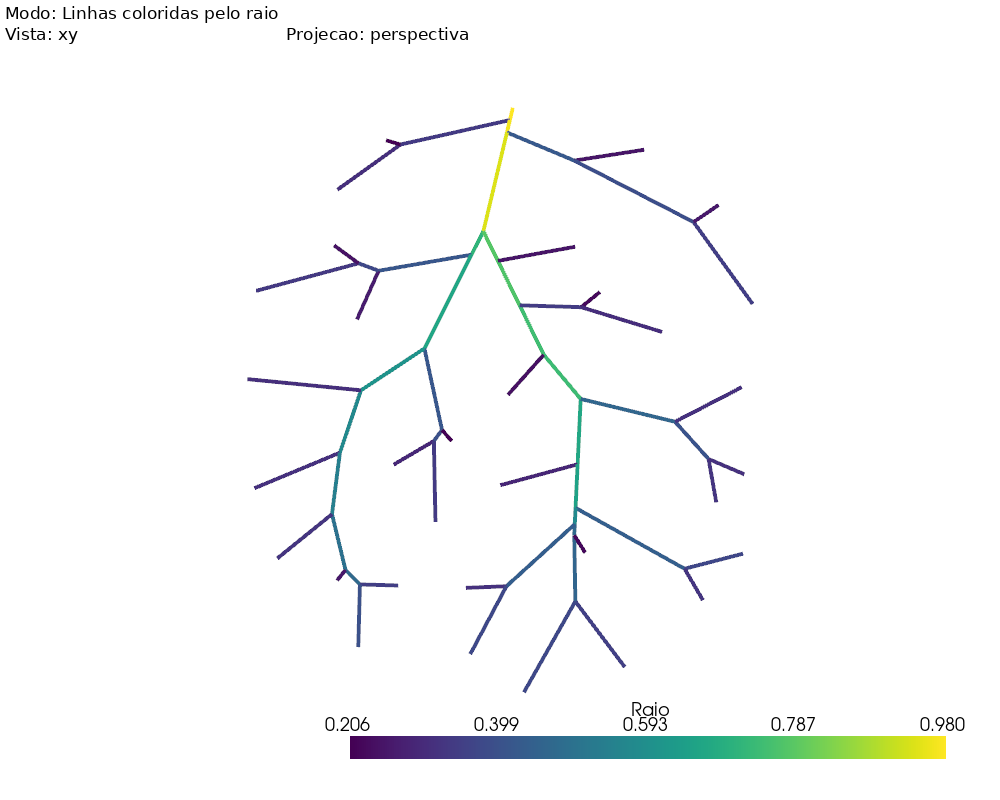
\includegraphics[width=\textwidth]{figures/modo0.png}
        \caption{Linhas coloridas pelo raio}
    \end{subfigure}
    \hfill
    \begin{subfigure}{0.32\textwidth}
        \centering
        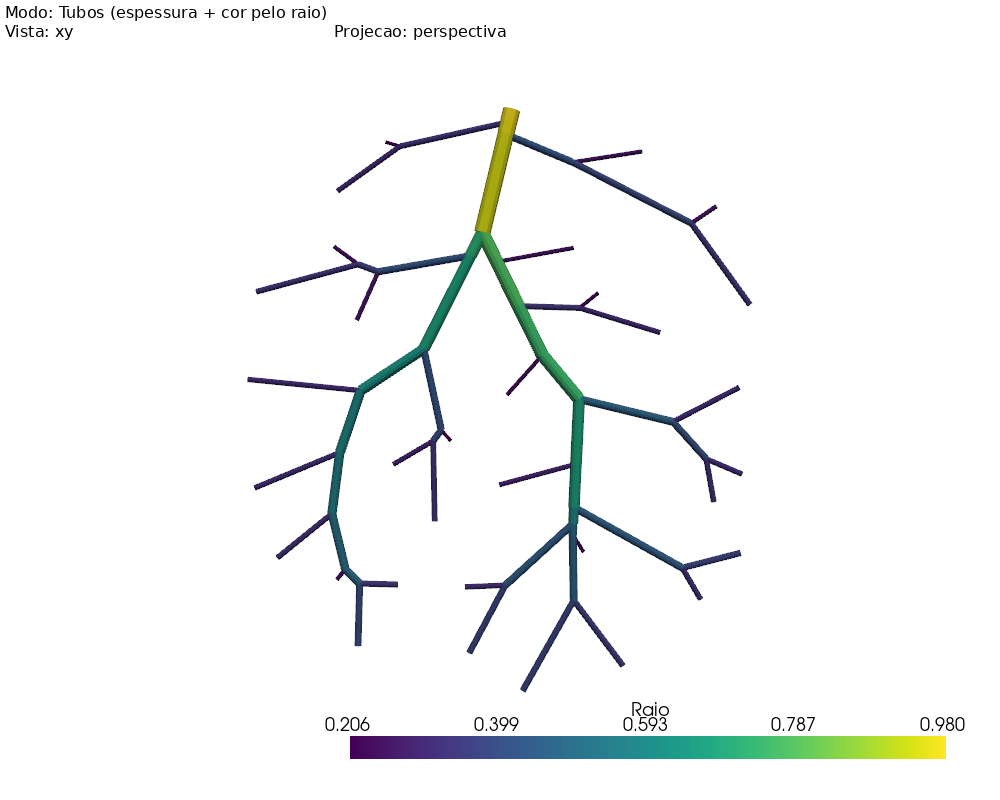
\includegraphics[width=\textwidth]{figures/modo1.png}
        \caption{Tubos com espessura e cor pelo raio}
    \end{subfigure}
    \hfill
    \begin{subfigure}{0.32\textwidth}
        \centering
        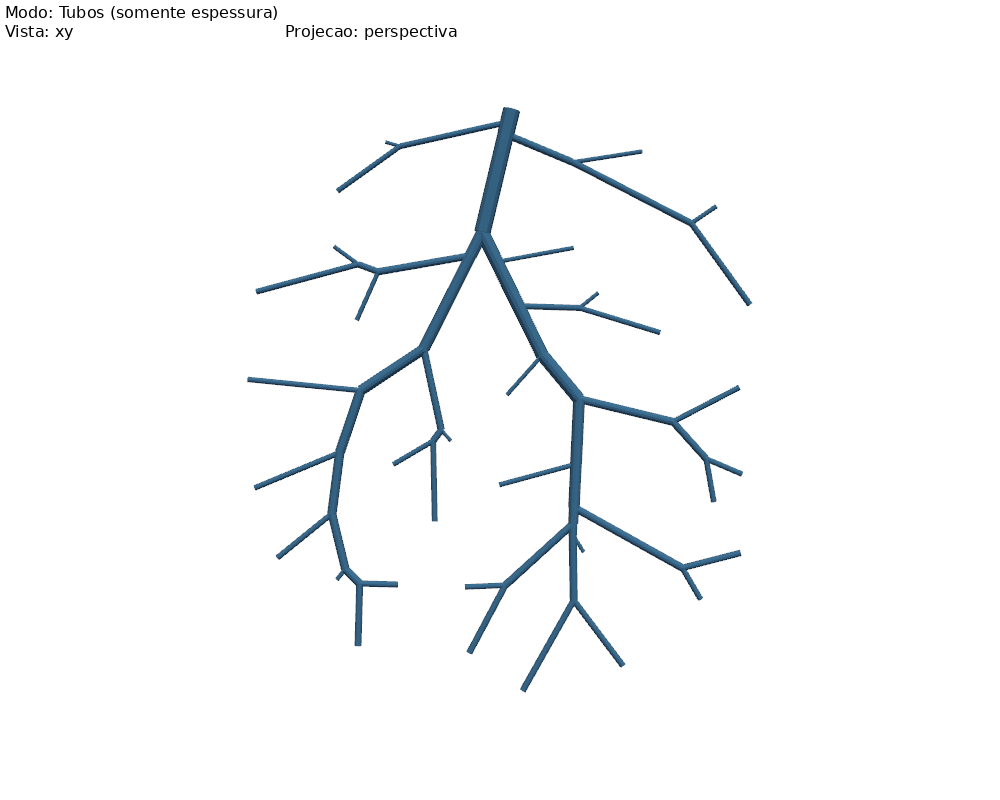
\includegraphics[width=\textwidth]{figures/modo2.png}
        \caption{Tubos apenas com espessura}
    \end{subfigure}

    \caption{Modos de representação das árvores: (a) linhas coloridas pelo raio; (b) tubos com espessura e cor pelo raio; (c) tubos apenas com espessura.}
    \label{fig:modos}
\end{figure}

\begin{figure}[htbp]
    \centering

    % Primeira linha
    \begin{subfigure}{0.32\textwidth}
        \centering
        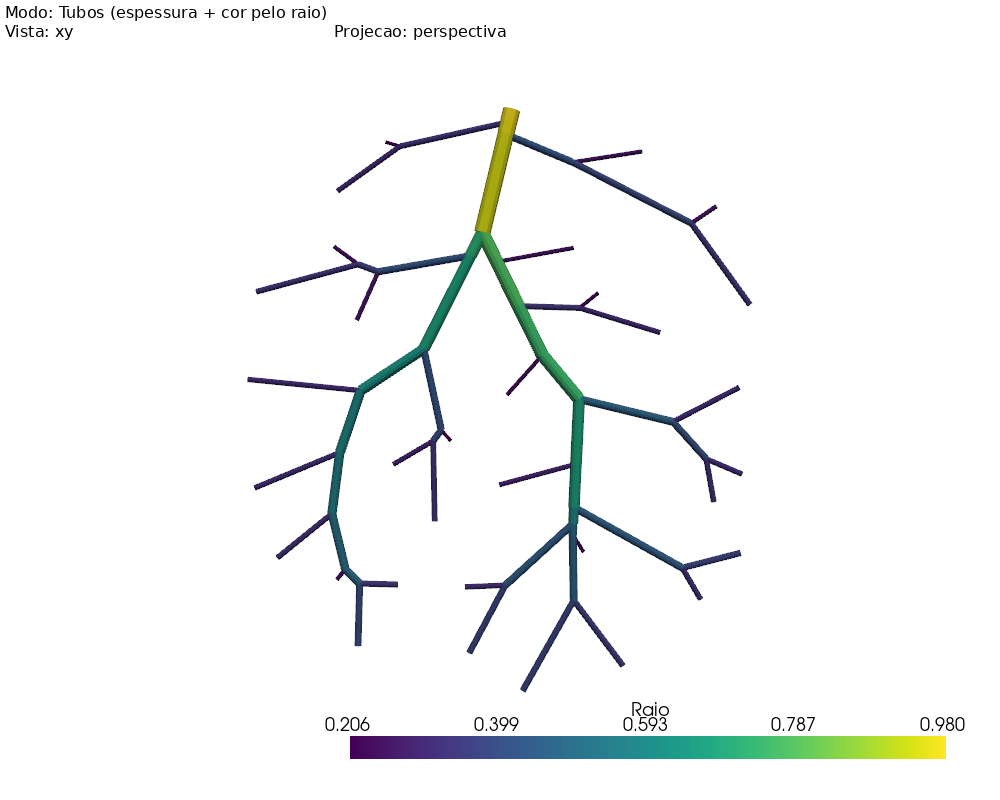
\includegraphics[width=\textwidth]{figures/vista0.png}
        \caption{Vista XY}
    \end{subfigure}
    \hfill
    \begin{subfigure}{0.32\textwidth}
        \centering
        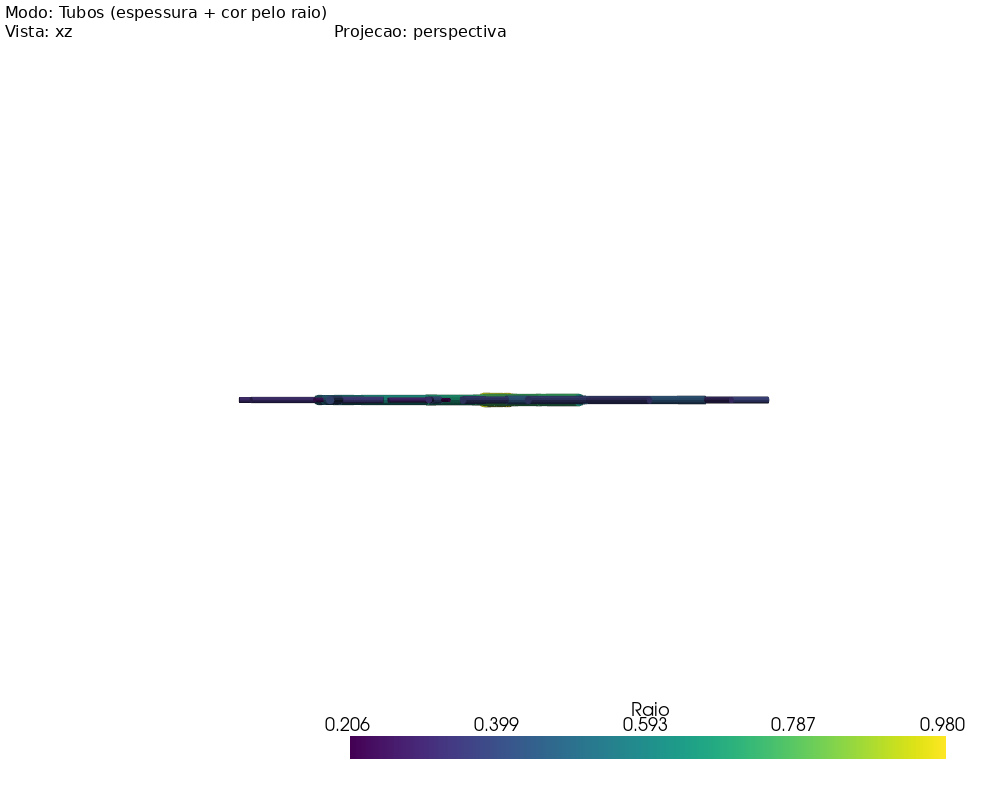
\includegraphics[width=\textwidth]{figures/vista1.png}
        \caption{Vista XZ}
    \end{subfigure}
    \hfill
    \begin{subfigure}{0.32\textwidth}
        \centering
        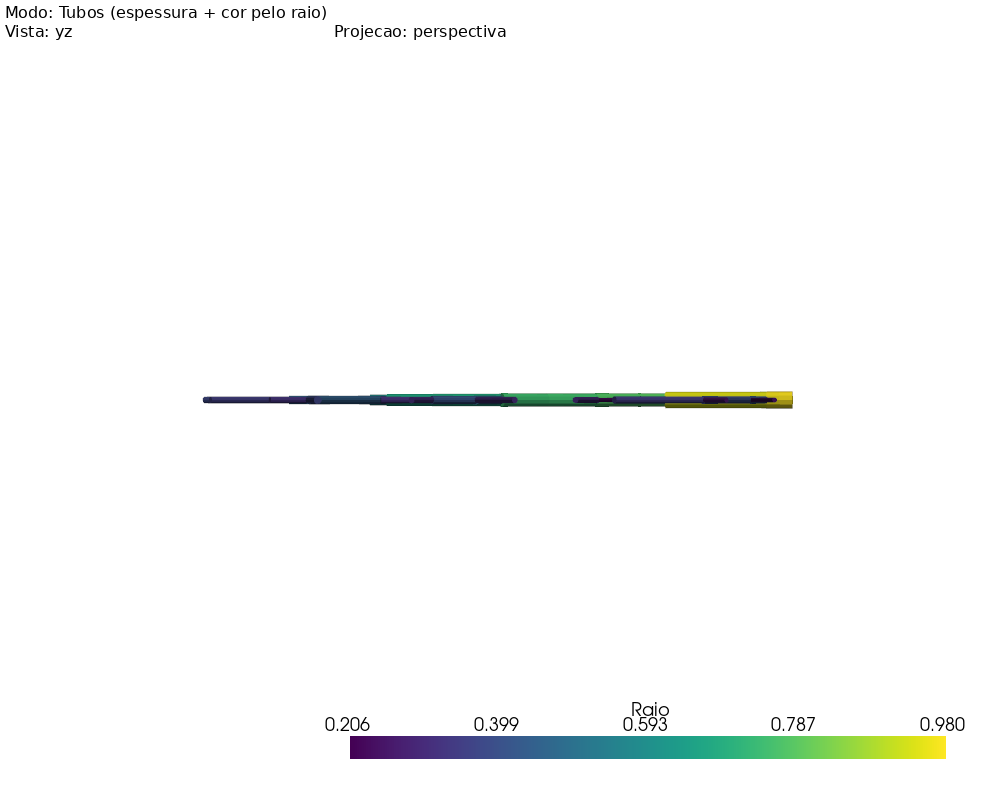
\includegraphics[width=\textwidth]{figures/vista2.png}
        \caption{Vista YZ}
    \end{subfigure}

    \vspace{0.3cm}

    % Segunda linha
    \begin{subfigure}{0.40\textwidth}
        \centering
        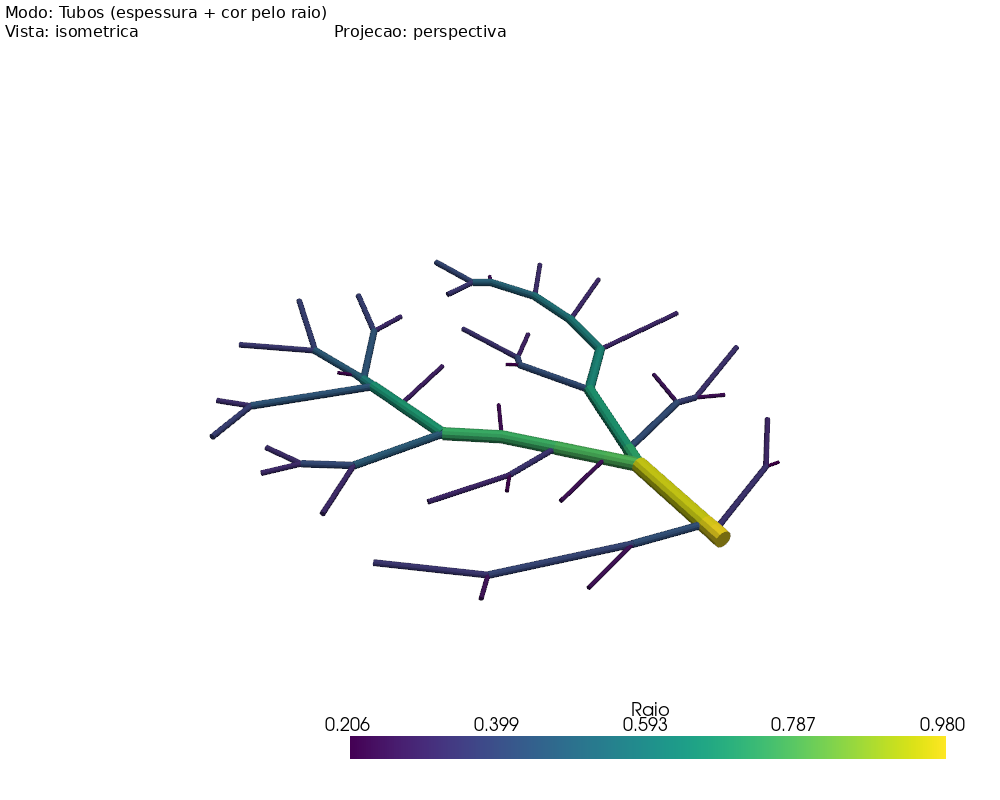
\includegraphics[width=\textwidth]{figures/vista3.png}
        \caption{Projeção em perspectiva com vista isometrica}
    \end{subfigure}
    \hspace{0.05\textwidth}
    \begin{subfigure}{0.40\textwidth}
        \centering
        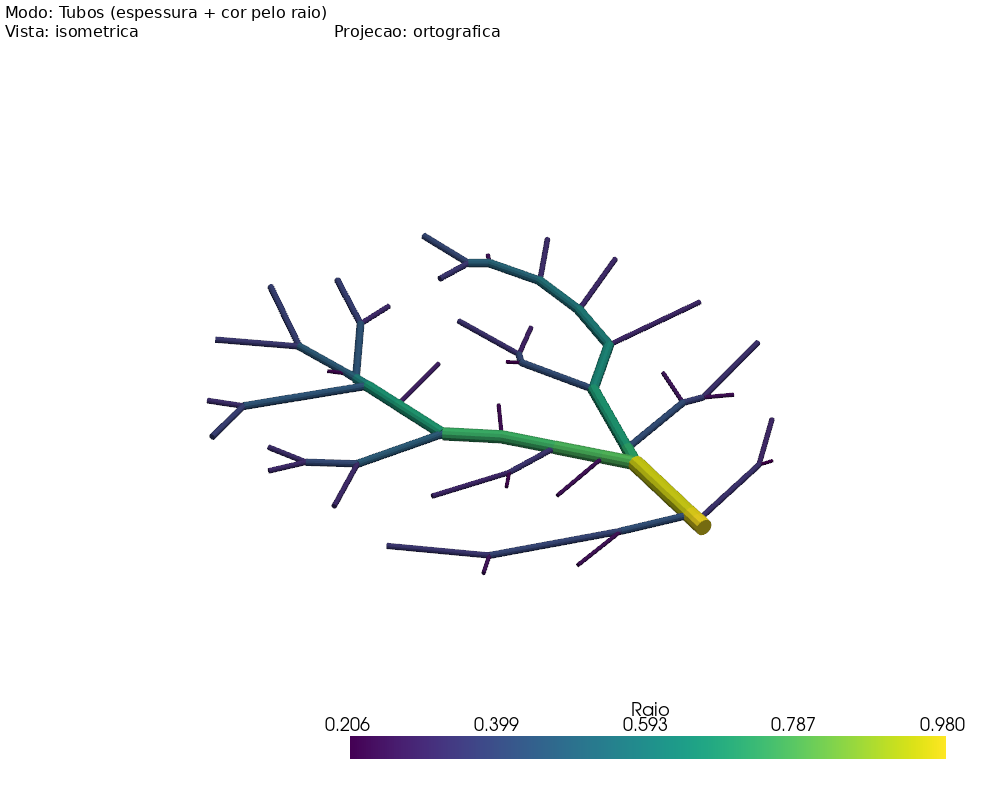
\includegraphics[width=\textwidth]{figures/vista4.png}
        \caption{Projeção ortográfica com vista isometrica}
    \end{subfigure}

    \caption{Observador em diferentes posições e comparação entre projeção ortográfica e perspectiva.}
    \label{fig:vistas}
\end{figure}

\noindent Como os modelos fornecidos são planos ($z=0$), a diferença entre as projeções só é visível quando o modelo é inclinado por rotações em $X$ ou $Y$ ou visto na vista isométrica. 

\subsection{Rasterização de linhas (Bresenham)}
\label{sec:res-bresenham}
A Tabela~\ref{tab:bresenham} traz o exemplo numérico do segmento $(0,0)\to(8,3)$, com $\Delta x=8$, $\Delta y=3$ e erro inicial $e=5$. Os 9 pixels gerados são $(0,0),(1,0),(2,1),(3,1),(4,1),(5,2),(6,2),(7,3),(8,3)$, e a Figura~\ref{fig:bres-ex} os compara com a reta ideal. A Figura~\ref{fig:bres-arv} mostra a árvore de 8 terminais rasterizada em $64\times64$ pixels (173 pixels pintados, com a cor de cada pixel dada pelo raio do vaso) e o detalhe do vaso 3.

\begin{table}[htbp]
  \centering
  \small
  \caption{Rastro do Bresenham para $(0,0)\to(8,3)$ (erro antes da decisão).}
  \label{tab:bresenham}
  \begin{tabular}{c|ccccccccc}
    \toprule
    \textbf{Passo} & 0 & 1 & 2 & 3 & 4 & 5 & 6 & 7 & 8 \\
    \midrule
    \textbf{Pixel} & (0,0) & (1,0) & (2,1) & (3,1) & (4,1) & (5,2) & (6,2) & (7,3) & (8,3) \\
    \textbf{Erro} & 5 & 2 & 7 & 4 & 1 & 6 & 3 & 8 & 5 \\
    \bottomrule
  \end{tabular}
\end{table}

\begin{figure}[htbp]
  \centering
  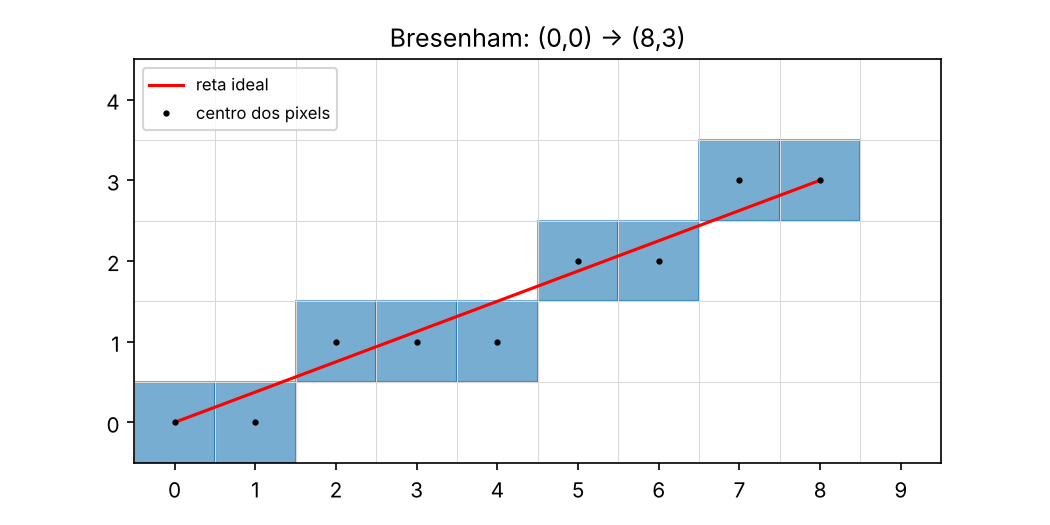
\includegraphics[width=0.62\textwidth]{figures/bresenham_exemplo.png}
  \caption{Pixels gerados pelo Bresenham para $(0,0)\to(8,3)$ e a reta ideal.}
  \label{fig:bres-ex}
\end{figure}

\begin{figure}[htbp]
  \centering
  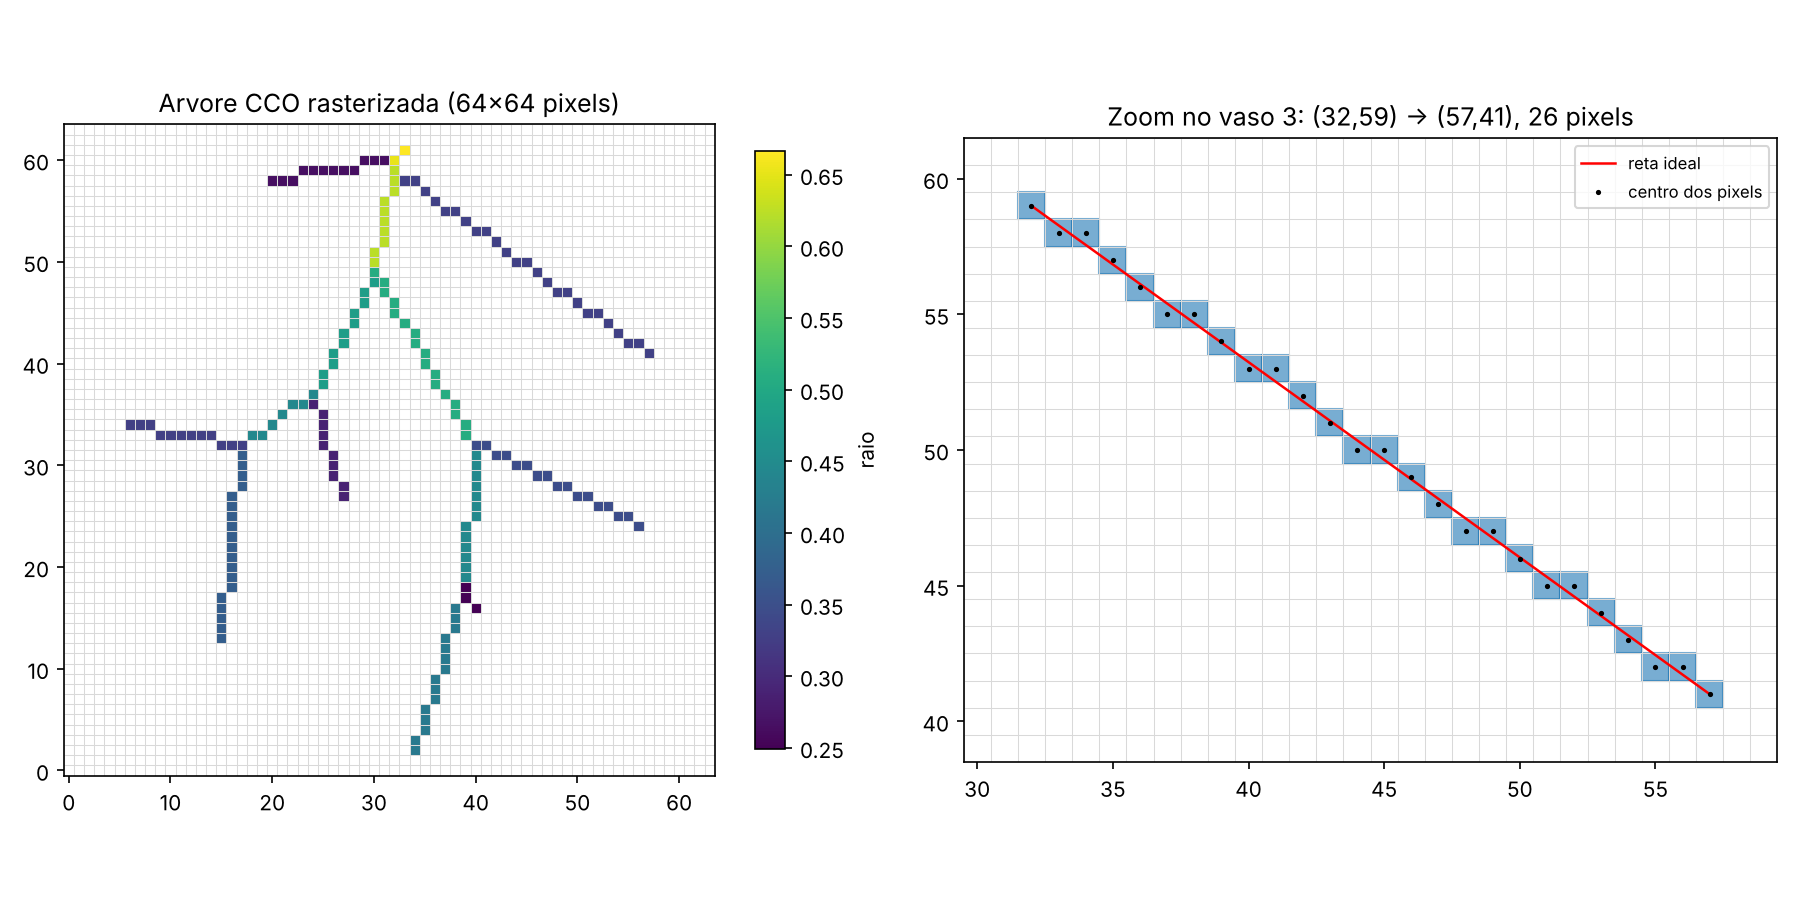
\includegraphics[width=\textwidth]{figures/bresenham_arvore.png}
  \caption{Árvore CCO de 8 terminais rasterizada em $64\times64$ pixels e detalhe de um vaso.}
  \label{fig:bres-arv}
\end{figure}

\subsection{Rasterização de polígonos (Scanline Fill)}
No polígono côncavo em U, a linha $y=12$ cruza as arestas em $x=2{,}5;\,8{,}5;\,15{,}5;\,21{,}5$, e são preenchidos os pares $(2{,}5;\,8{,}5)$ e $(15{,}5;\,21{,}5)$, o que deixa a cavidade do U sem pintura. O preenchimento resulta em 222 pixels, igual à área esperada. A região de interesse hexagonal sobre a árvore ocupa 732 pixels. A Figura~\ref{fig:scan} mostra os dois casos.

\begin{figure}[htbp]
  \centering
  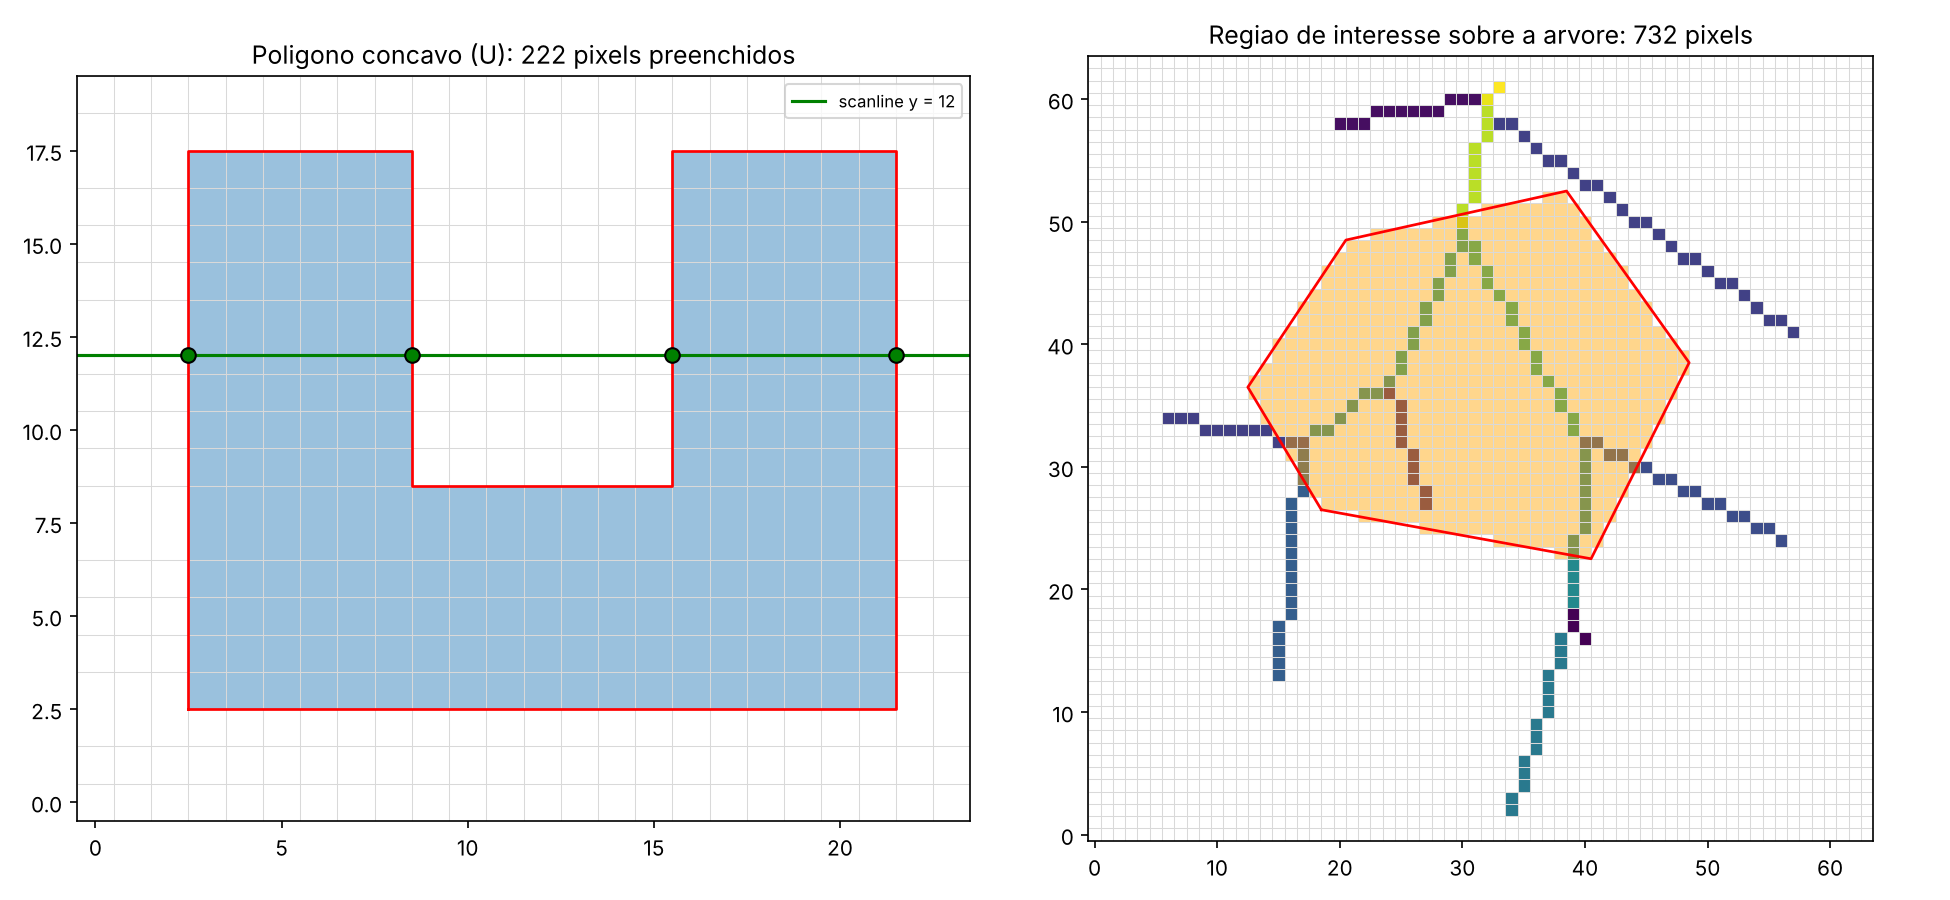
\includegraphics[width=\textwidth]{figures/scanline_fill.png}
  \caption{Scanline Fill: polígono côncavo com uma linha de varredura destacada e região de interesse sobre a árvore.}
  \label{fig:scan}
\end{figure}

Como polígono auxiliar mais relacionado ao modelo, tomou-se a raiz e as 8 folhas da árvore, ordenadas pelo ângulo em torno do centroide, o que gera um polígono simples (verificado por teste de cruzamento de arestas) e possivelmente côncavo. O preenchimento resultou em 1695 pixels, contra a área exata de 1693,3 pela fórmula do cadarço (Figura~\ref{fig:scan-ext}).

\begin{figure}[htbp]
  \centering
  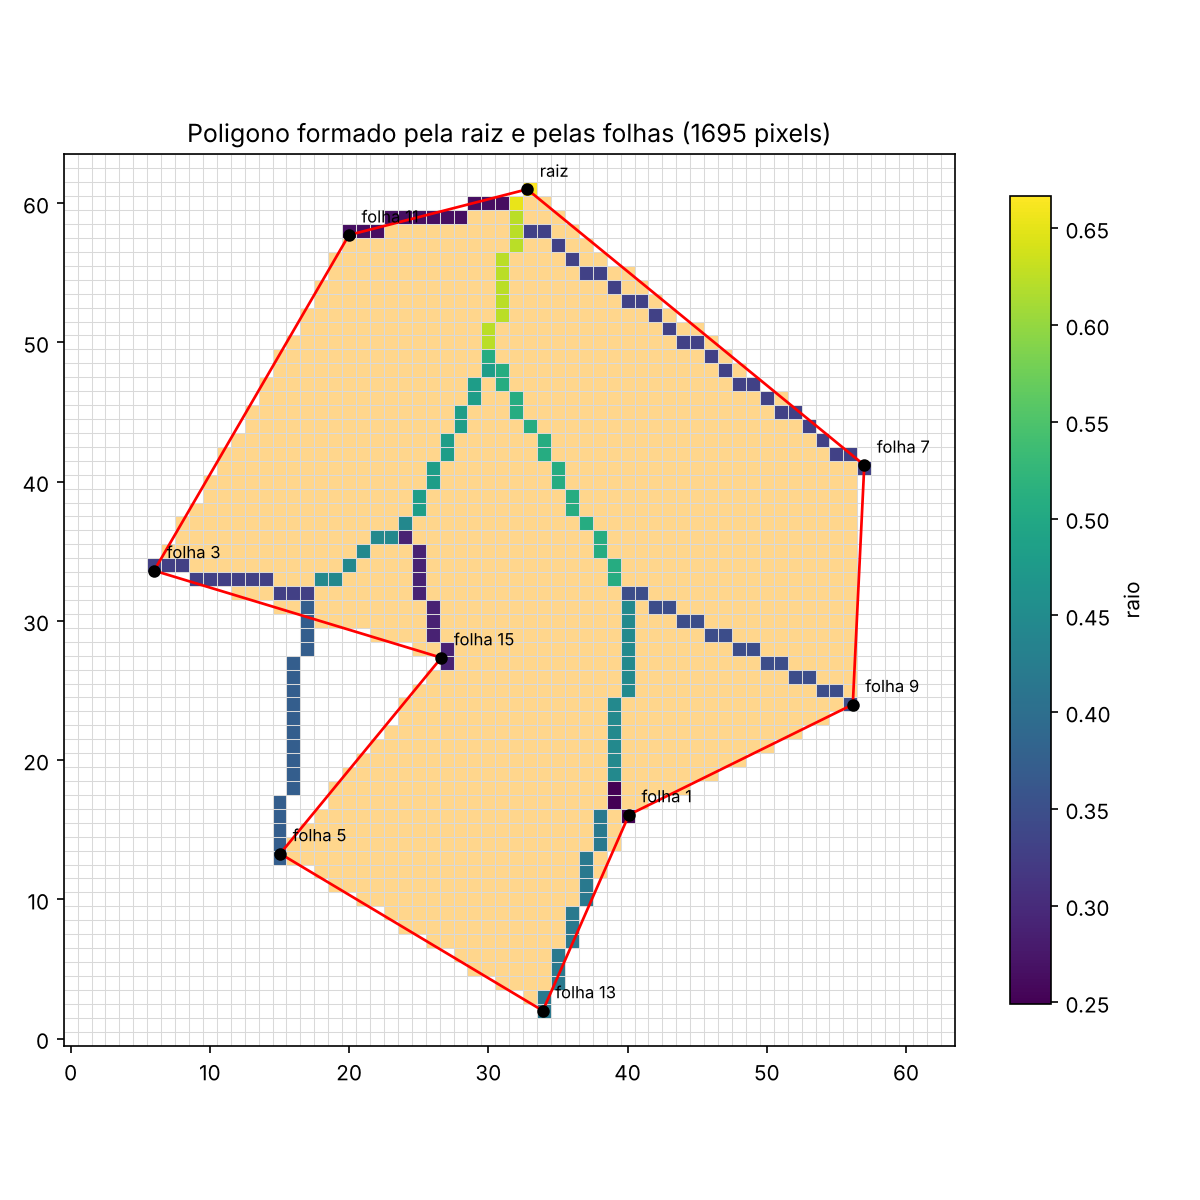
\includegraphics[width=0.62\textwidth]{figures/scanline_extremos.png}
  \caption{Polígono formado pela raiz e pelas folhas da árvore, preenchido pelo Scanline Fill.}
  \label{fig:scan-ext}
\end{figure}

\subsection{Aliasing e antialiasing}
\label{sec:res-aa}
A Figura~\ref{fig:aa} compara a renderização com uma amostra por pixel e com \emph{supersampling} $4\times4$ (16 amostras por pixel), com detalhe ampliado nas linhas inclinadas. Sem antialiasing, os traços diagonais aparecem em degraus e a imagem tem apenas 17 tons distintos de luminância; com $k=4$, as bordas ganham tons intermediários e há 200 tons distintos. Como medida objetiva, a Tabela~\ref{tab:aa} traz o erro quadrático médio (EQM) em relação a uma referência de $16\times16$ amostras. O EQM cai de forma consistente com $k$, e o ganho é mais forte entre $k=1$ e $k=4$.

\begin{figure}[htbp]
  \centering
  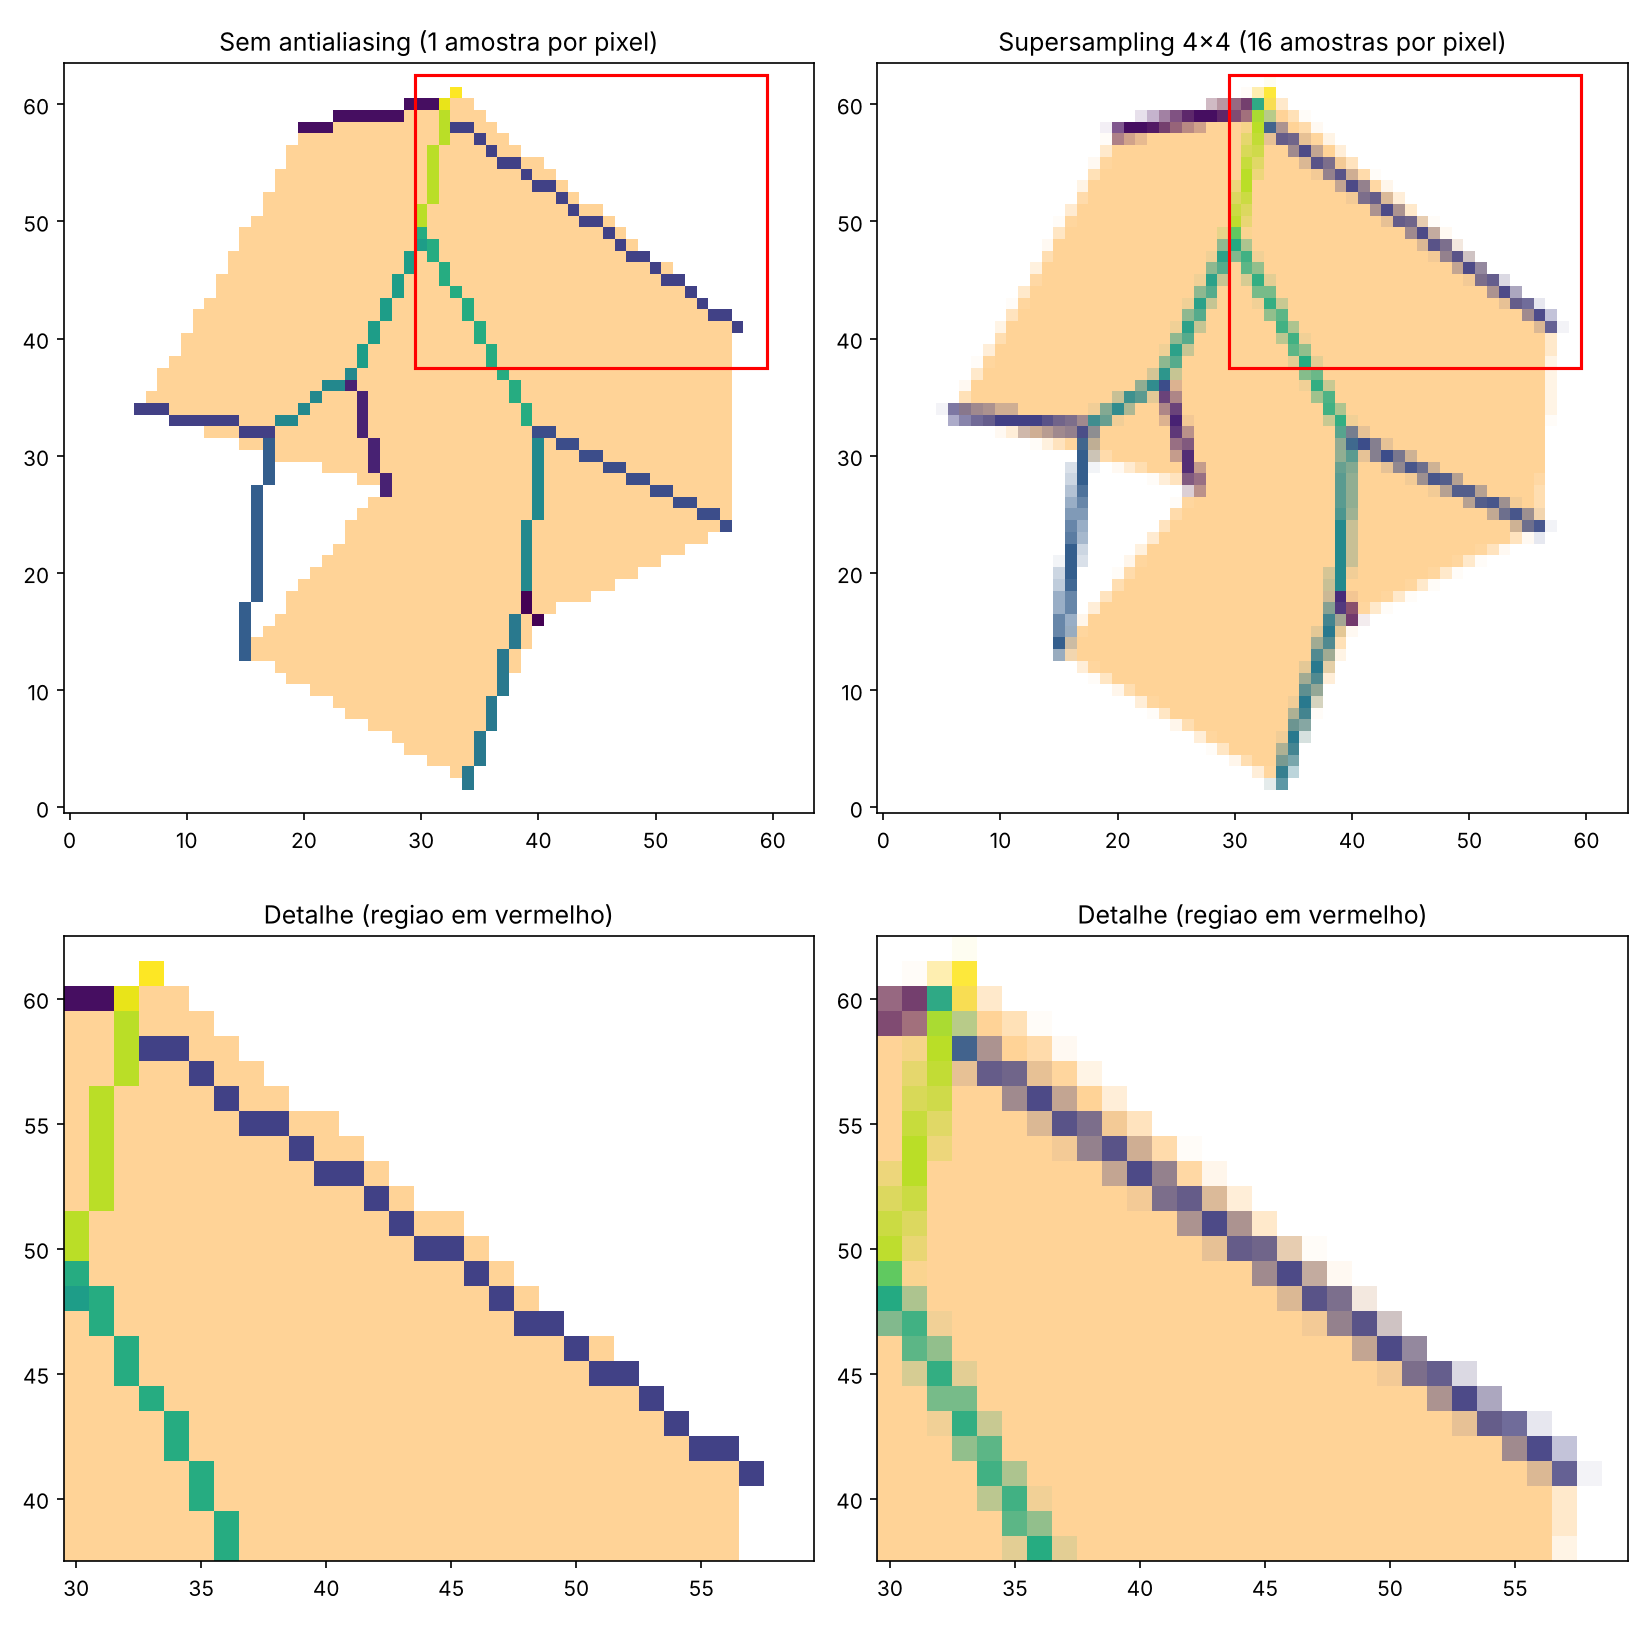
\includegraphics[width=0.82\textwidth]{figures/antialiasing.png}
  \caption{Sem antialiasing e com \emph{supersampling} $4\times4$ (linha superior) e detalhe da região em vermelho (linha inferior).}
  \label{fig:aa}
\end{figure}

\begin{table}[htbp]
  \centering
  \small
  \caption{EQM em relação à referência com $16\times16$ amostras por pixel (grade $64\times64$).}
  \label{tab:aa}
  \begin{tabular}{lcccc}
    \toprule
    \textbf{Fator} $k$ & 1 (sem AA) & 2 & 4 & 8 \\
    \midrule
    \textbf{Amostras por pixel} & 1 & 4 & 16 & 64 \\
    \textbf{EQM} & $4{,}68\times10^{-3}$ & $1{,}72\times10^{-3}$ & $2{,}4\times10^{-4}$ & $3\times10^{-5}$ \\
    \bottomrule
  \end{tabular}
\end{table}

\subsection{Recorte de segmentos}
O exemplo numérico adota a janela $x\in[2,8]$, $y\in[2,6]$ e o segmento $(-1,7)\to(10,1)$. O Cohen--Sutherland precisa de quatro recortes (Tabela~\ref{tab:cs}): os extremos começam nas regiões \texttt{1001} (acima e à esquerda) e \texttt{0110} (abaixo e à direita) e terminam em $(2;\,5{,}364)$ e $(8;\,2{,}091)$. O Liang--Barsky chega ao mesmo trecho em quatro passos (Tabela~\ref{tab:lb}): $t_0=0{,}2727$, vindo da borda esquerda, e $t_1=0{,}8182$, vindo da direita. A Figura~\ref{fig:rec-ex} ilustra os códigos de região e os recortes sucessivos.

\begin{table}[htbp]
  \centering
  \small
  \caption{Cohen--Sutherland no exemplo: extremos e códigos (ACIMA ABAIXO DIREITA ESQUERDA) a cada iteração.}
  \label{tab:cs}
  \begin{tabular}{cllcc}
    \toprule
    \textbf{Iteração} & \textbf{$P_0$} & \textbf{Código de $P_0$} & \textbf{$P_1$} & \textbf{Código de $P_1$} \\
    \midrule
    0 & $(-1{,}000;\,7{,}000)$ & 1001 & $(10{,}000;\,1{,}000)$ & 0110 \\
    1 & $(0{,}833;\,6{,}000)$ & 0001 & $(10{,}000;\,1{,}000)$ & 0110 \\
    2 & $(2{,}000;\,5{,}364)$ & 0000 & $(10{,}000;\,1{,}000)$ & 0110 \\
    3 & $(2{,}000;\,5{,}364)$ & 0000 & $(8{,}167;\,2{,}000)$ & 0010 \\
    4 & $(2{,}000;\,5{,}364)$ & 0000 & $(8{,}000;\,2{,}091)$ & 0000 \\
    \bottomrule
  \end{tabular}
\end{table}

\begin{table}[htbp]
  \centering
  \small
  \caption{Liang--Barsky no mesmo exemplo.}
  \label{tab:lb}
  \begin{tabular}{lrrrl}
    \toprule
    \textbf{Borda} & $p$ & $q$ & $t$ & \textbf{Efeito} \\
    \midrule
    esquerda & $-11{,}00$ & $-3{,}00$ & $0{,}2727$ & entra: $t_0=0{,}2727$ \\
    direita & $11{,}00$ & $9{,}00$ & $0{,}8182$ & sai: $t_1=0{,}8182$ \\
    abaixo & $6{,}00$ & $5{,}00$ & $0{,}8333$ & sai: $t_1=0{,}8182$ \\
    acima & $-6{,}00$ & $-1{,}00$ & $0{,}1667$ & entra: $t_0=0{,}2727$ \\
    \bottomrule
  \end{tabular}
\end{table}

\begin{figure}[htbp]
  \centering
  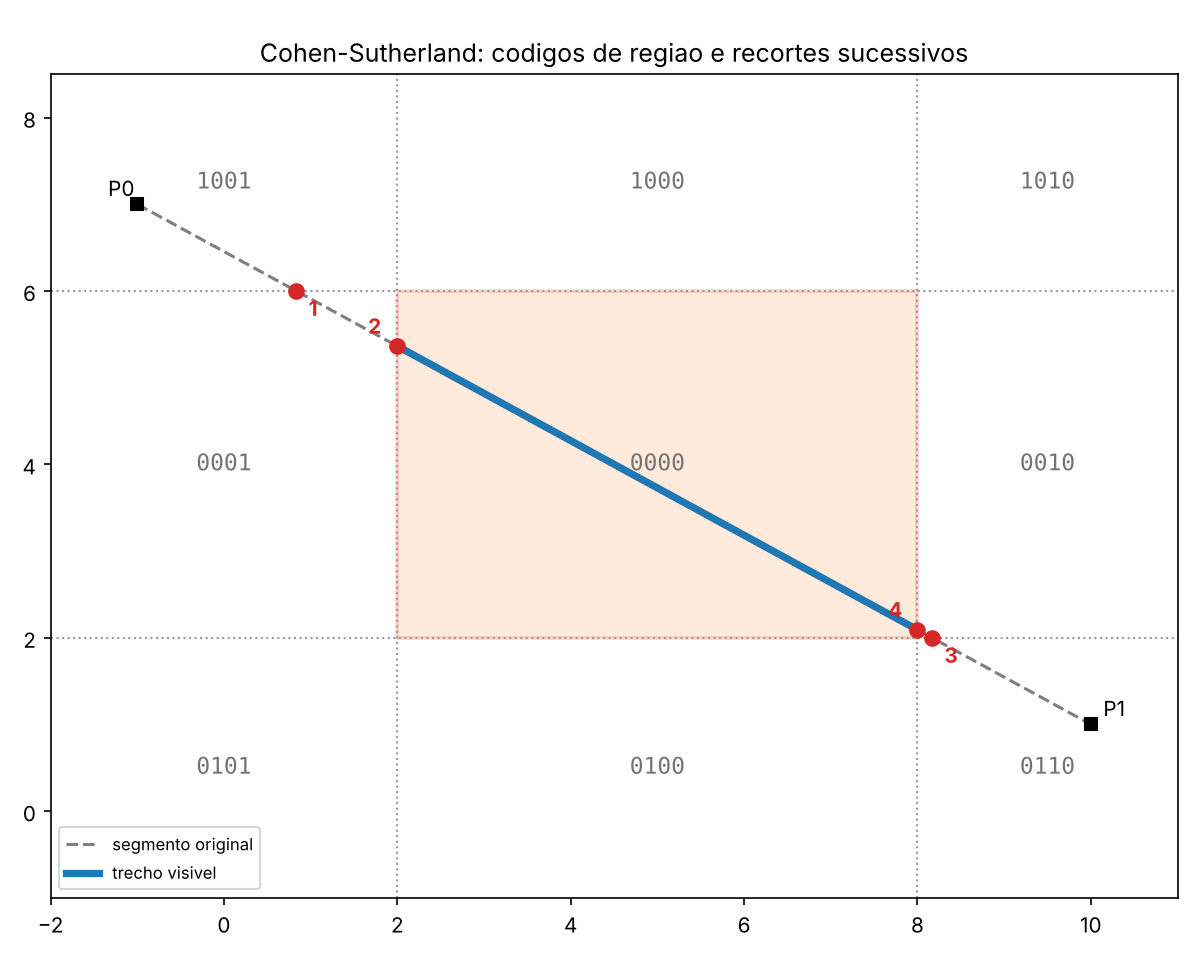
\includegraphics[width=0.55\textwidth]{figures/recorte_exemplo.png}
  \caption{Cohen--Sutherland: códigos de região e recortes sucessivos (pontos numerados).}
  \label{fig:rec-ex}
\end{figure}

Sobre a árvore de 8 terminais, a janela escolhida automaticamente foi $x\in[-0{,}0280;\,0{,}0150]$ e $y\in[-0{,}0047;\,0{,}0450]$. Dos 15 segmentos, 3 foram aceitos trivialmente, 4 rejeitados trivialmente, 8 recortados e nenhum rejeitado após recortes, o que deixa 11 trechos visíveis. Na grade $64\times64$, o número de pixels pintados passou de 173 para 76. Cohen--Sutherland e Liang--Barsky produziram exatamente a mesma imagem (0 pixels diferentes). A Figura~\ref{fig:rec-arv} traz as imagens antes e depois do recorte.

\begin{figure}[htbp]
  \centering
  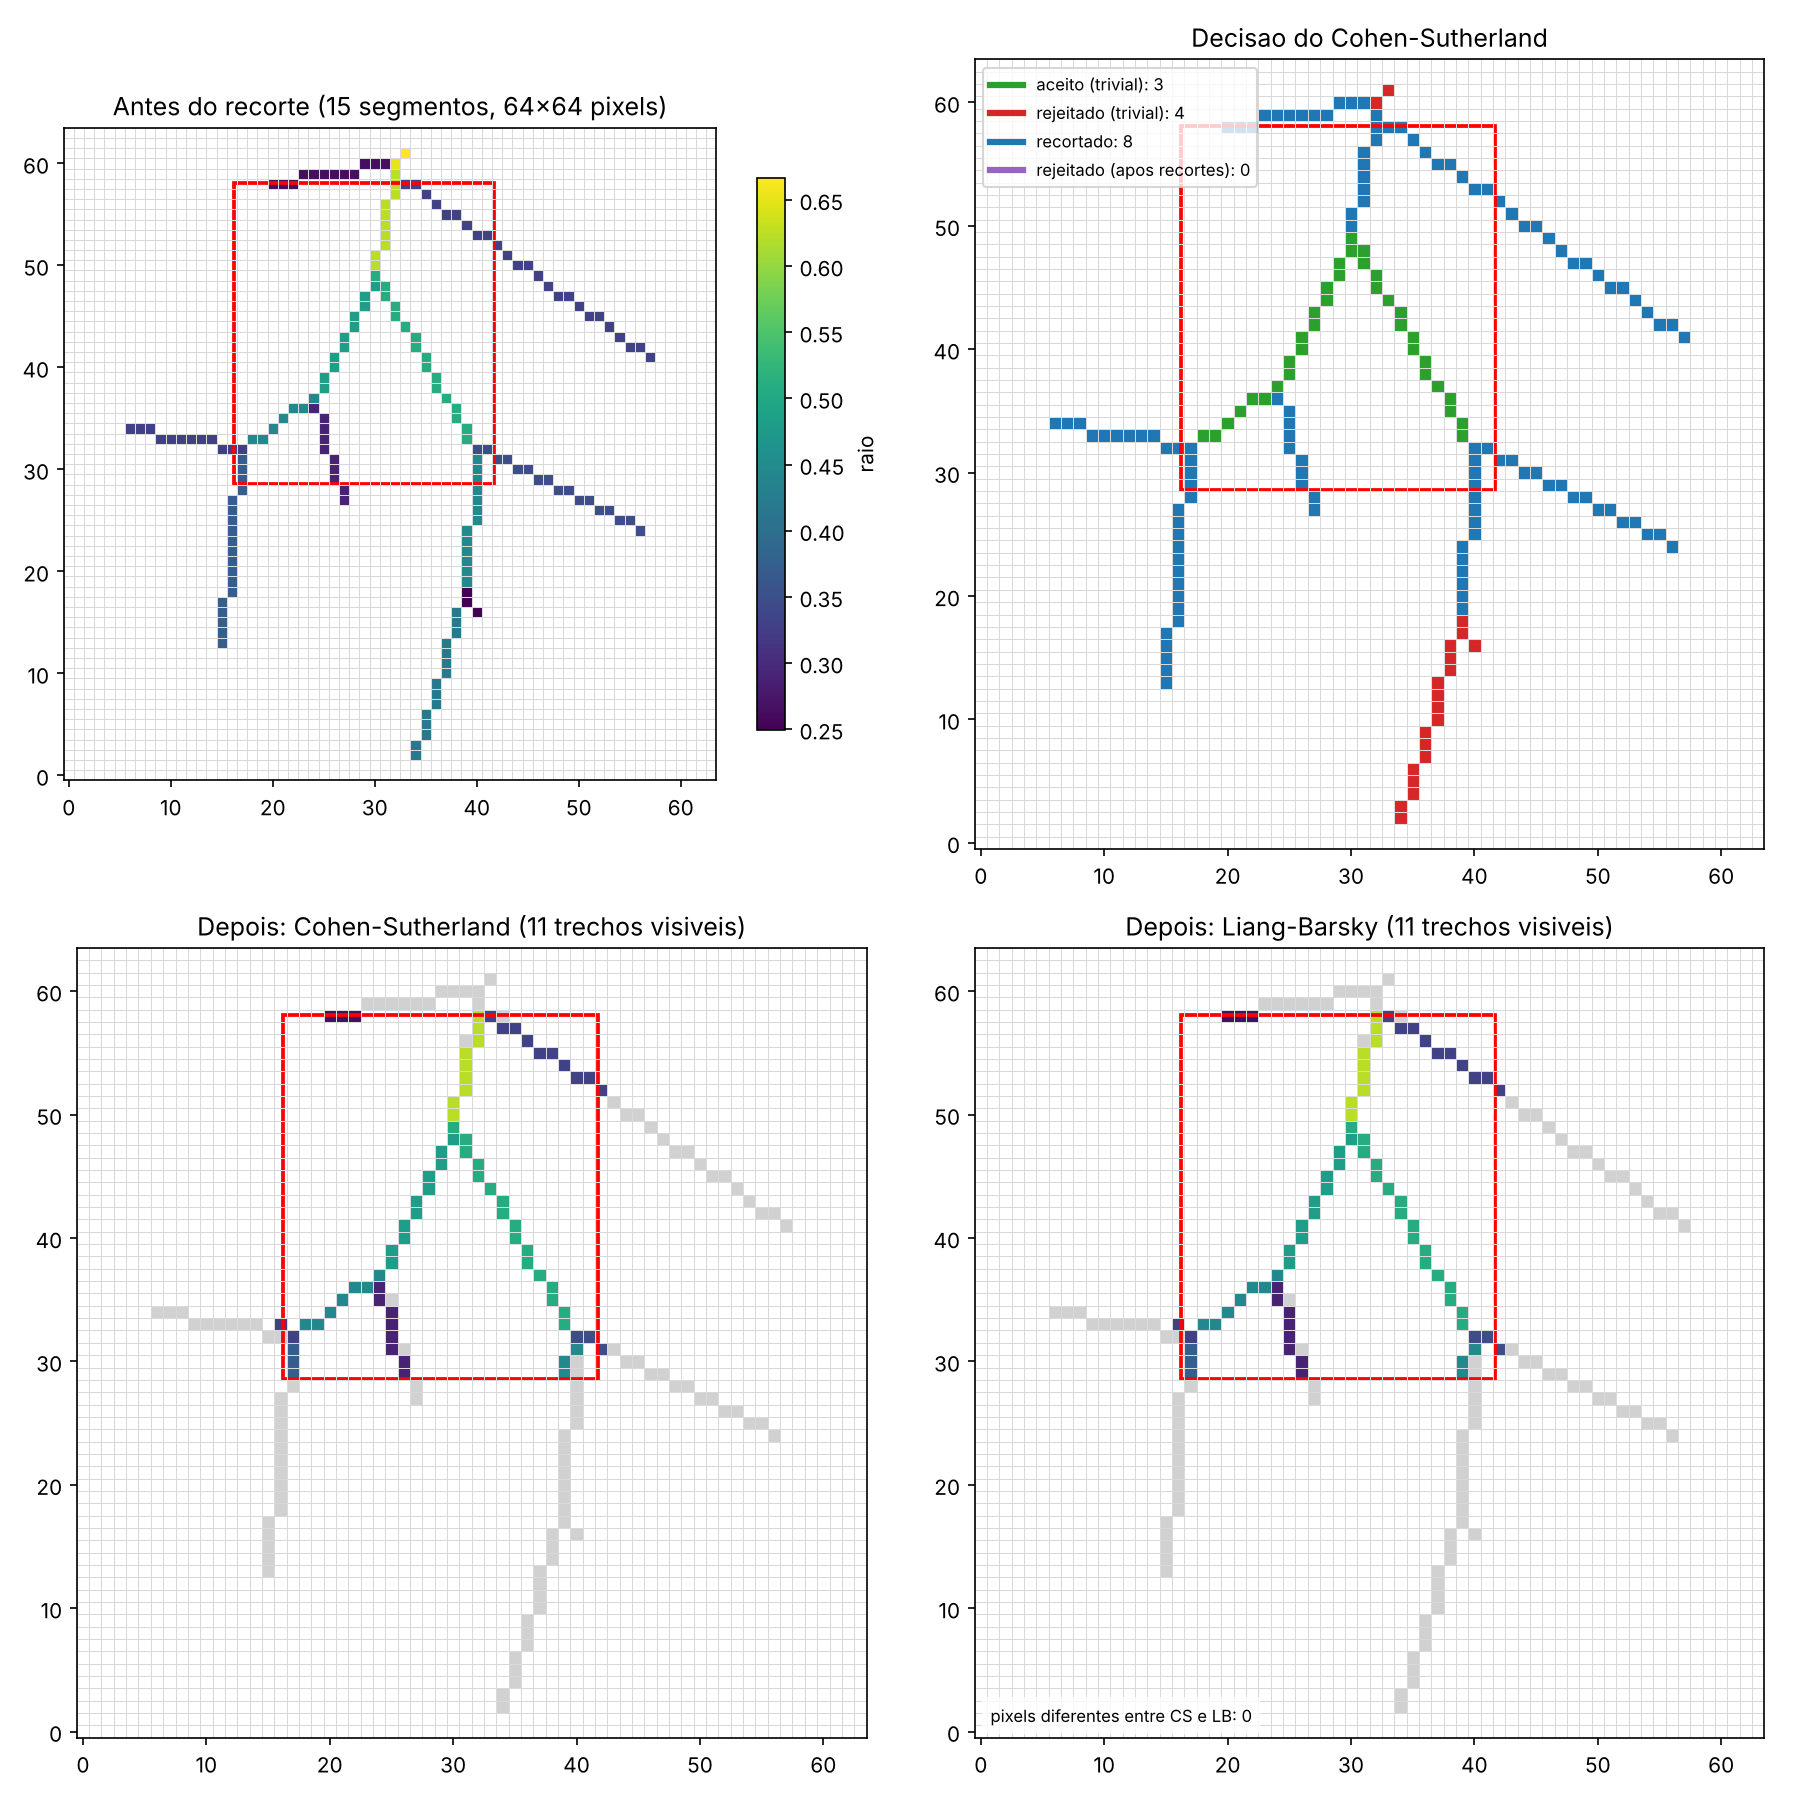
\includegraphics[width=0.88\textwidth]{figures/recorte_arvore.png}
  \caption{Recorte da árvore: antes, decisão do Cohen--Sutherland e depois (Cohen--Sutherland e Liang--Barsky).}
  \label{fig:rec-arv}
\end{figure}

Para comparar o custo, os dois algoritmos foram cronometrados em 20\,000 segmentos aleatórios no quadrado $[-1,2]^2$ contra a janela $[0,1]^2$ (melhor de três execuções, Python puro): o Cohen--Sutherland levou cerca de 17,6~ms e o Liang--Barsky cerca de 43,3~ms, valores estáveis em repetições. Nesse conjunto, 39,1\% dos segmentos foram rejeitados trivialmente, 51,2\% recortados, 8,3\% rejeitados após recortes e 1,4\% aceitos. \todo{Repetir a medição na máquina do grupo e atualizar os valores, que dependem do hardware.}

\subsection{Recorte de polígonos}
A Figura~\ref{fig:sh-ex} mostra o Sutherland--Hodgman em um quadrilátero de vértices $(3{,}5;\,9{,}5)$, $(11{,}5;\,2{,}5)$, $(20{,}5;\,9{,}5)$ e $(13{,}5;\,18{,}5)$ contra a janela $x\in[7{,}5;\,17{,}5]$, $y\in[5{,}5;\,14{,}5]$. A cada borda aplicada, o número de vértices evolui $4\to5\to6\to7\to8$, e o resultado final tem 8 vértices e área de 86,47 (fórmula do cadarço).

\begin{figure}[htbp]
  \centering
  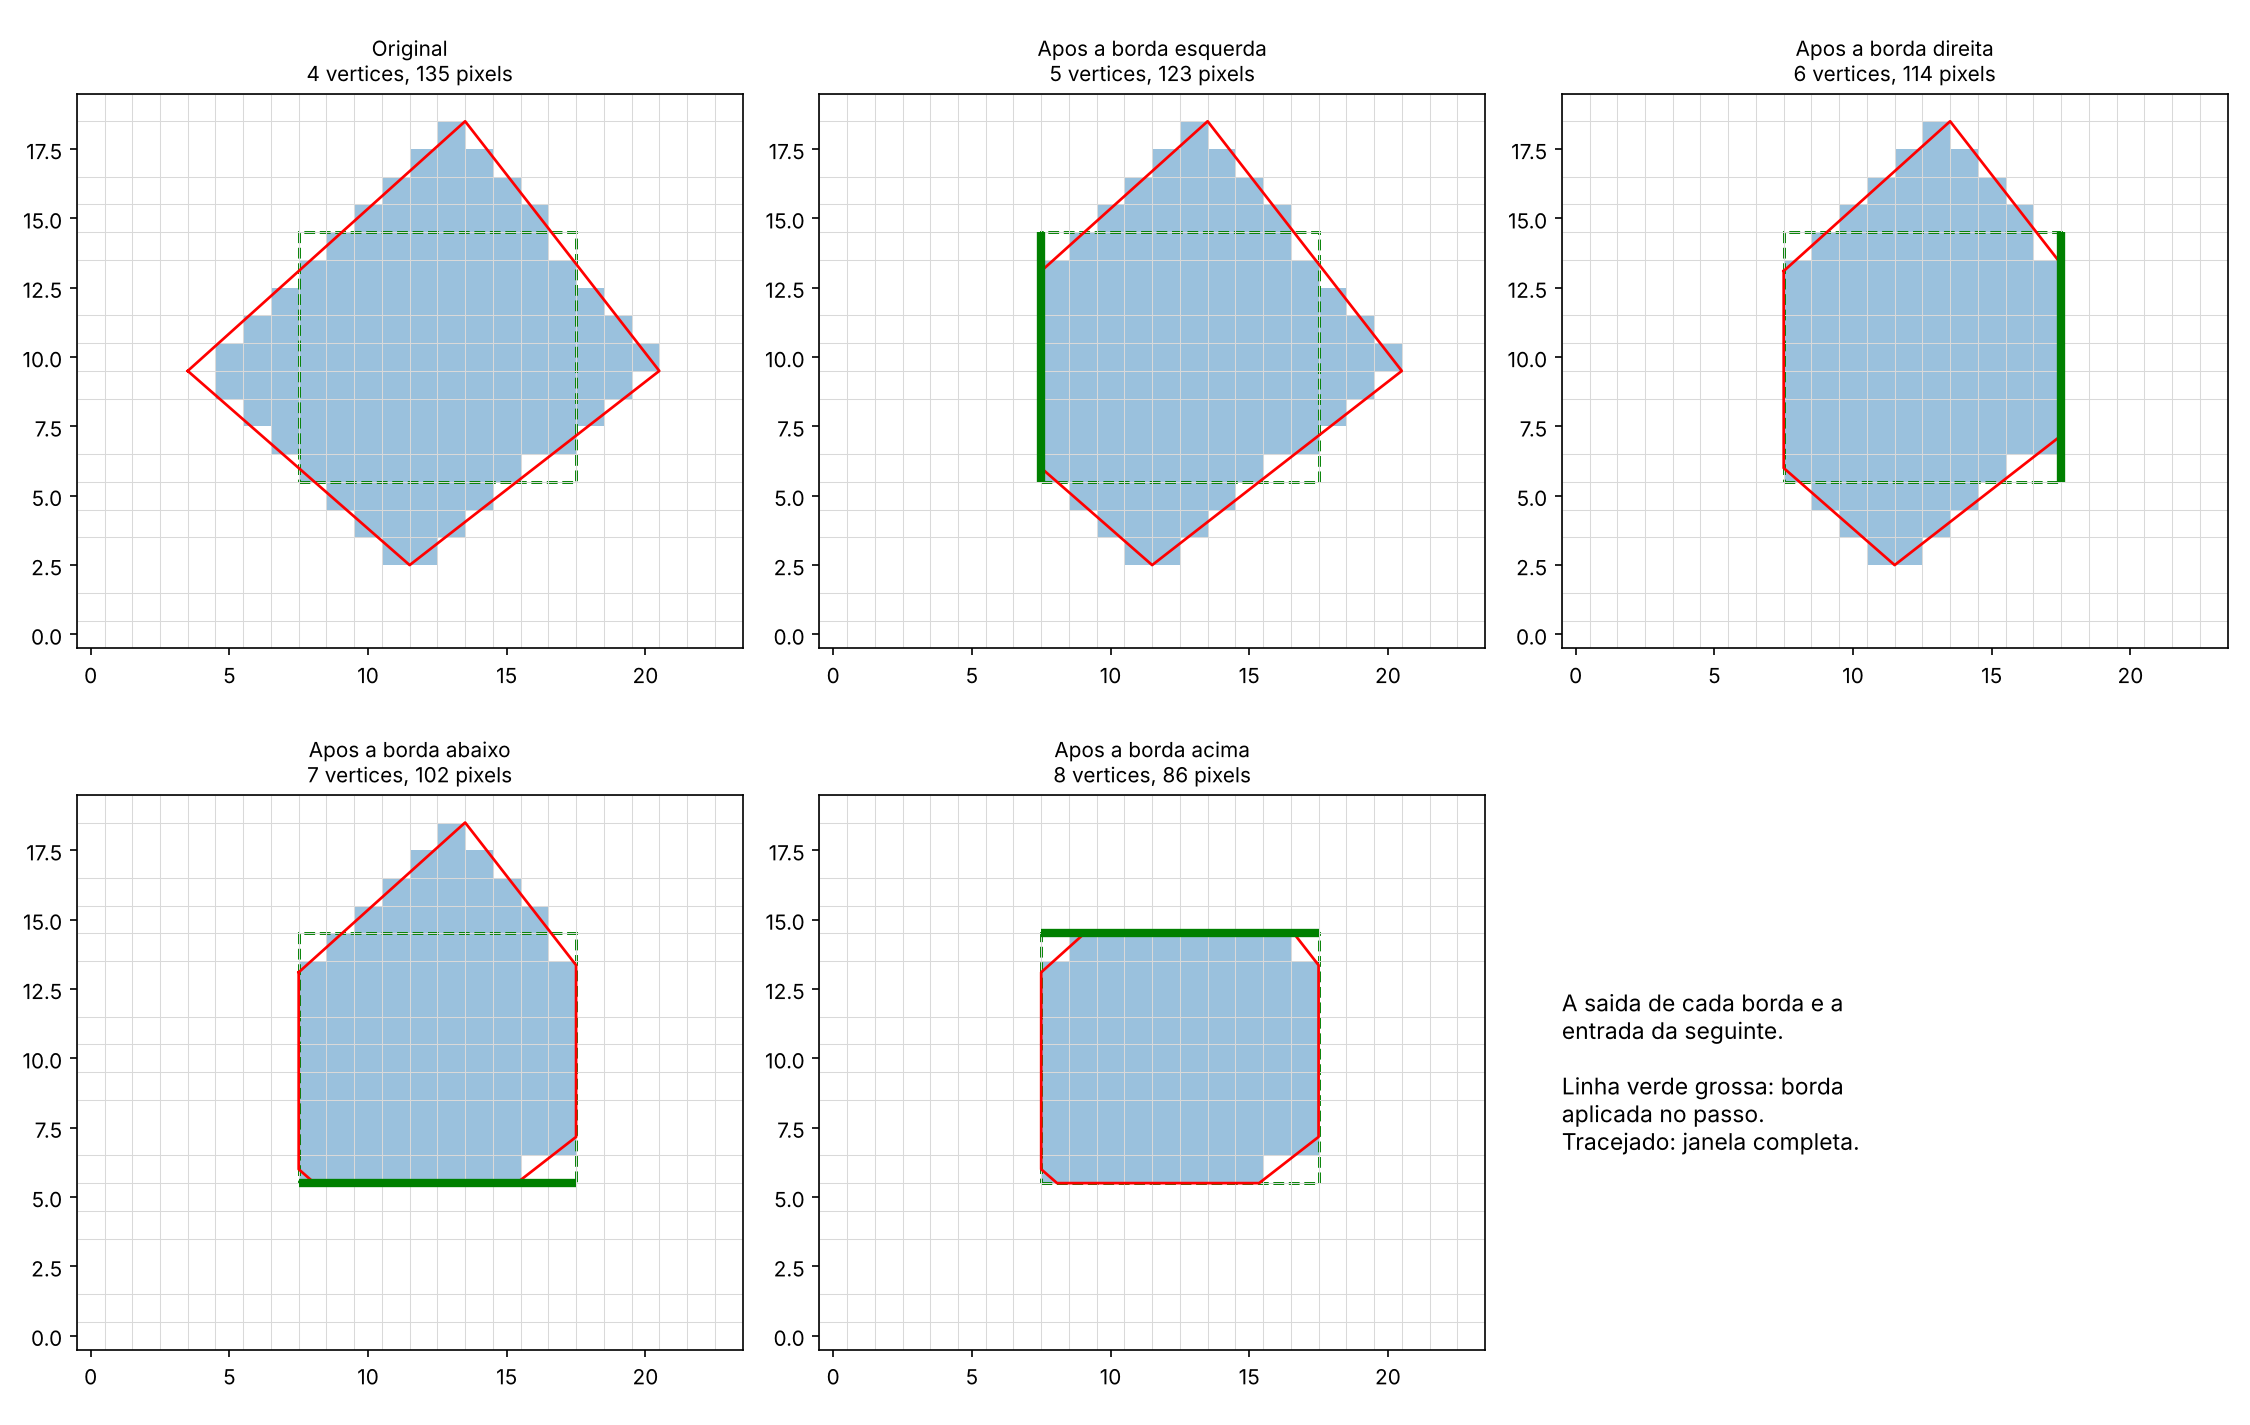
\includegraphics[width=\textwidth]{figures/recorte_poligono_exemplo.png}
  \caption{Sutherland--Hodgman passo a passo: o polígono é recortado contra uma borda por vez.}
  \label{fig:sh-ex}
\end{figure}

O polígono côncavo em U mostra uma limitação do algoritmo (Figura~\ref{fig:sh-conc}). Recortado por $y\ge10{,}5$, o resultado correto são dois braços separados, mas a saída é uma única lista de 8 vértices, em que os dois pedaços ficam ligados por um trecho de borda, de $(8{,}5;\,10{,}5)$ a $(15{,}5;\,10{,}5)$, percorrido nos dois sentidos. O preenchimento por par-ímpar ainda gera os 84 pixels corretos (conferidos com o teste do raio), mas o polígono não é ``limpo''.

\begin{figure}[htbp]
  \centering
  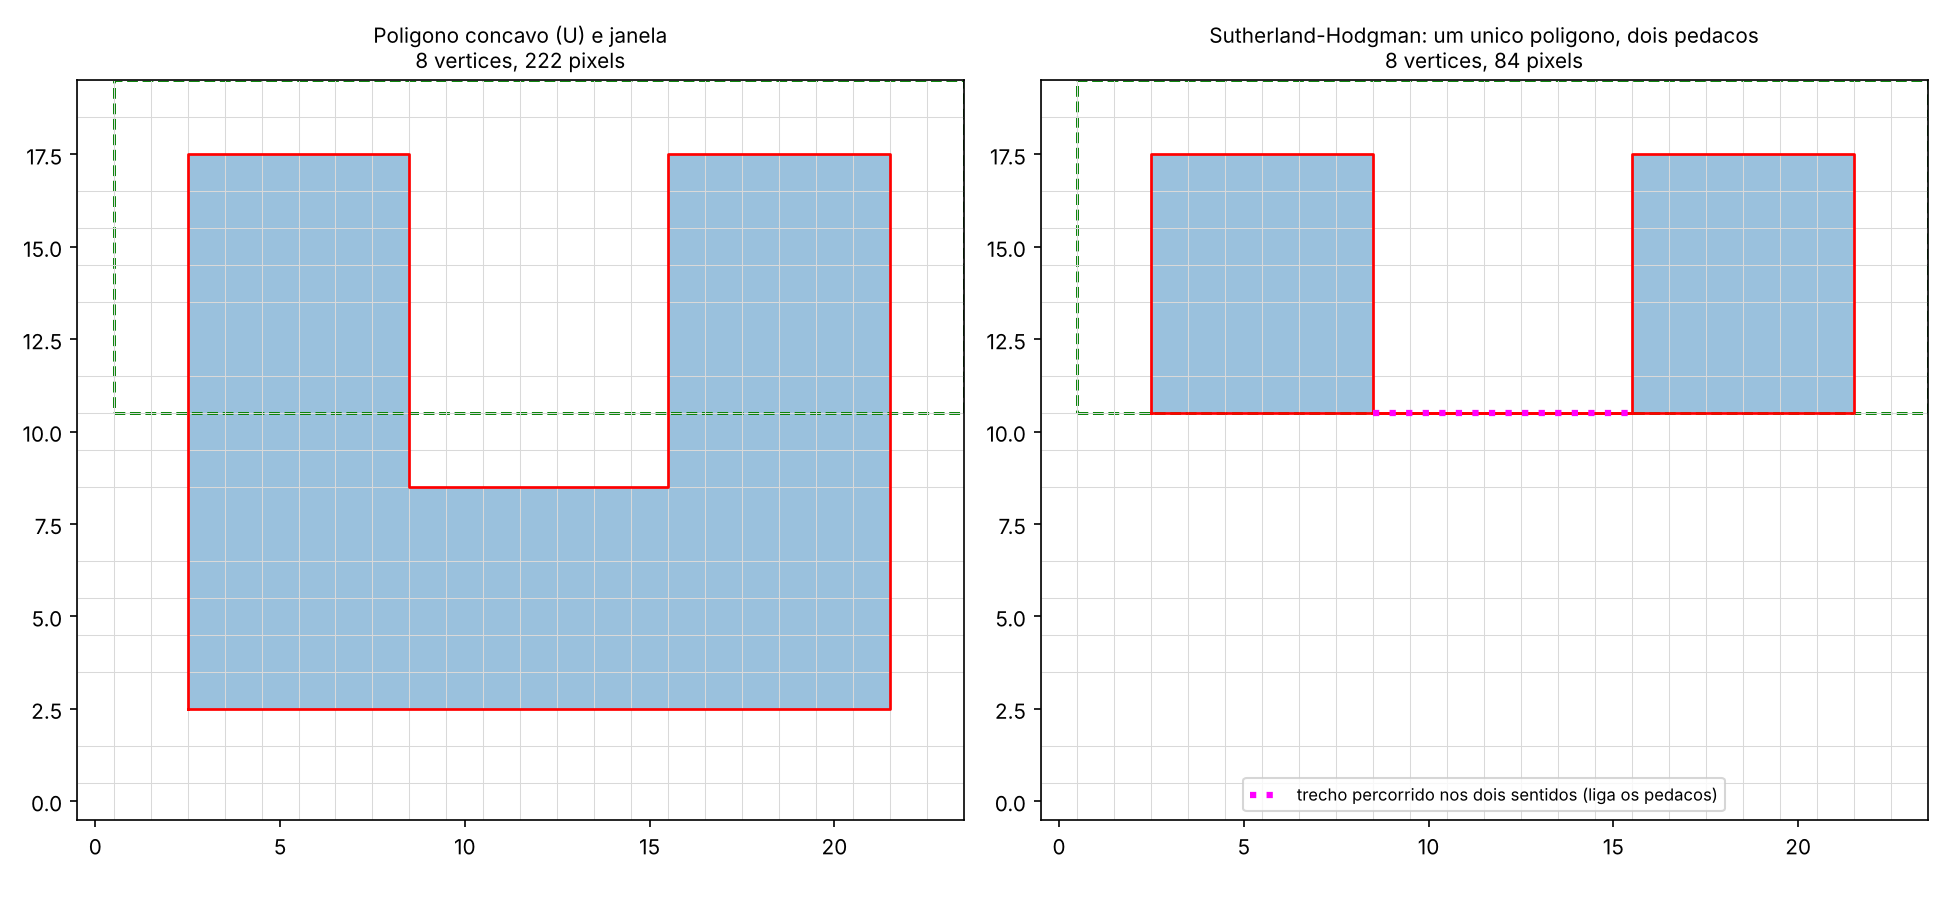
\includegraphics[width=\textwidth]{figures/recorte_poligono_concavo.png}
  \caption{Polígono côncavo em U recortado: um único polígono com dois pedaços ligados sobre a borda.}
  \label{fig:sh-conc}
\end{figure}

Aplicado ao polígono da raiz e das folhas da árvore, o recorte pela mesma janela do exemplo anterior reduziu o polígono de 9 vértices e 1695 pixels para 8 vértices e 717 pixels, sem trechos sobrepostos (Figura~\ref{fig:sh-arv}).

\begin{figure}[htbp]
  \centering
  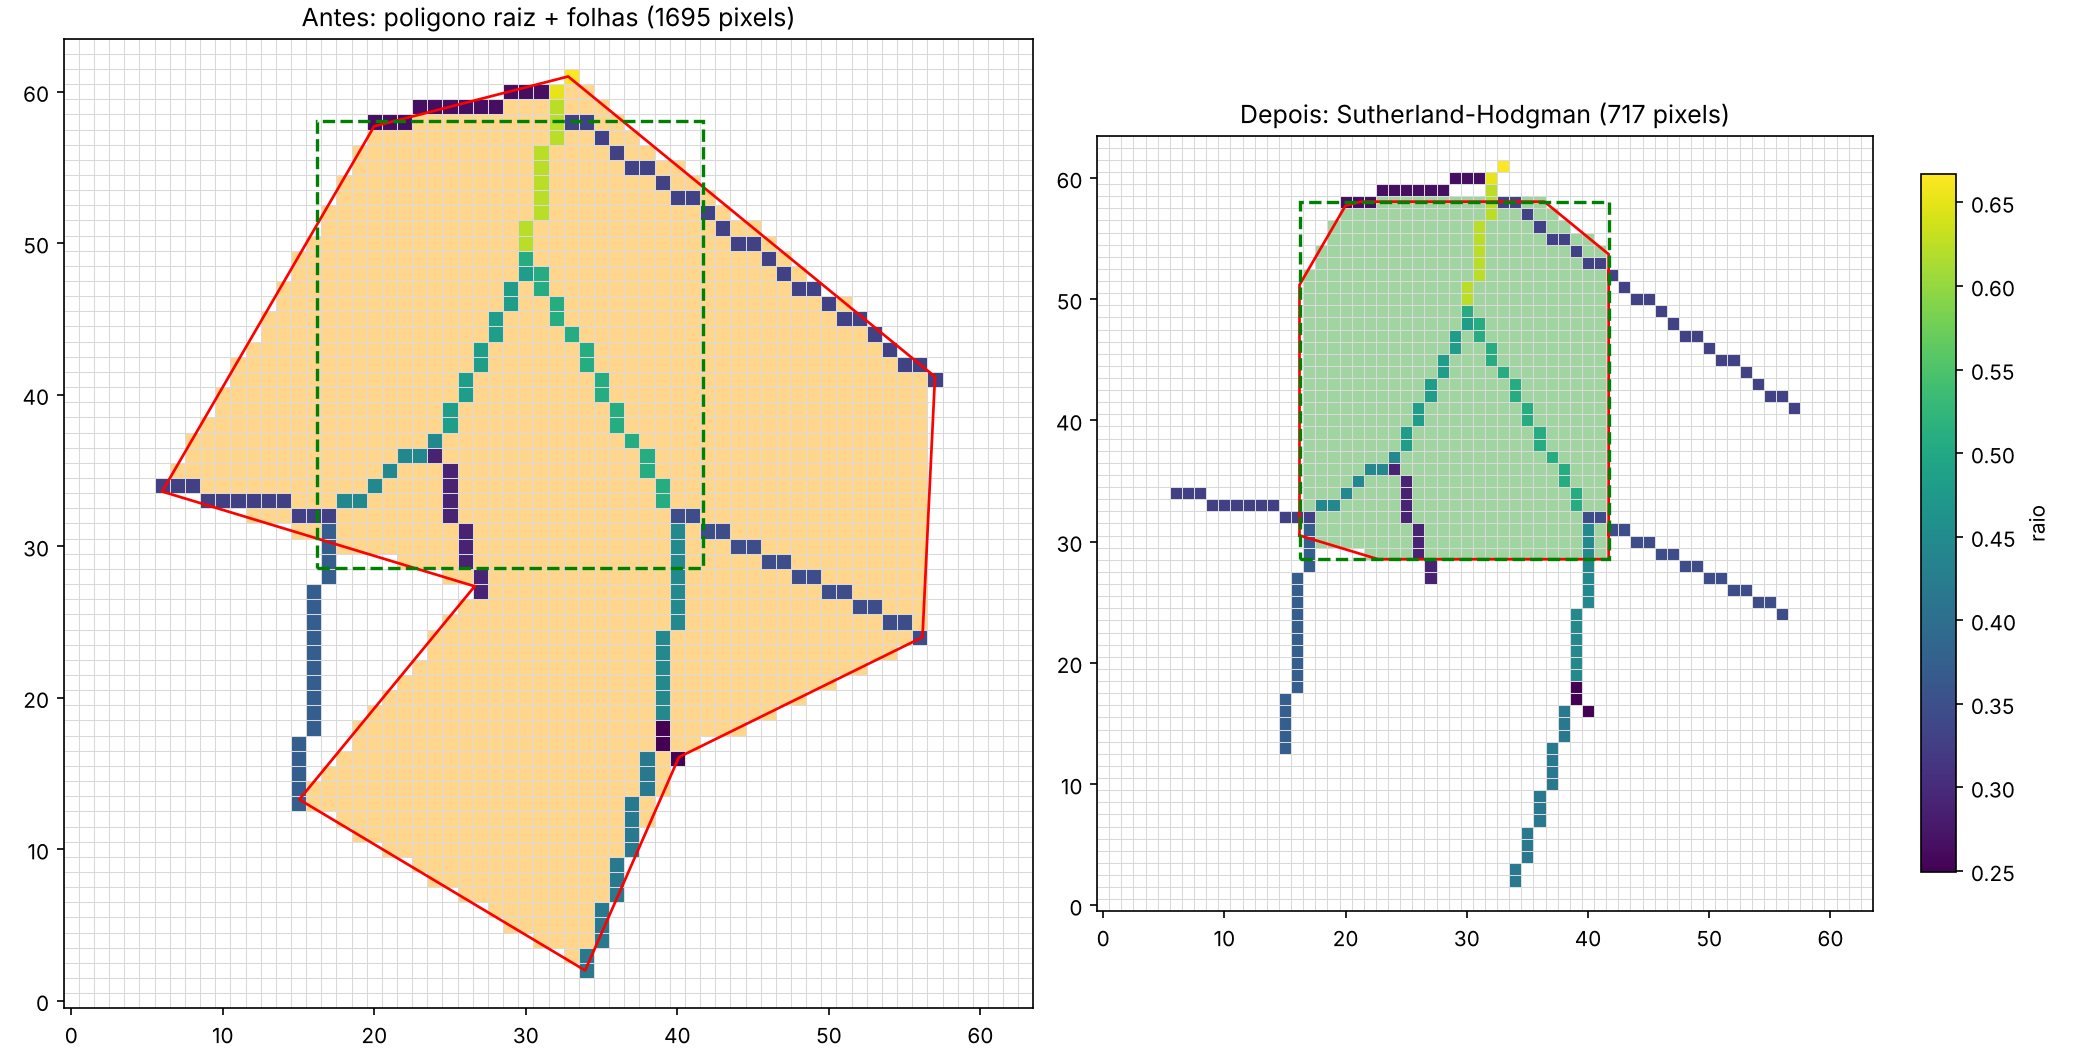
\includegraphics[width=\textwidth]{figures/recorte_poligono_arvore.png}
  \caption{Polígono da raiz e das folhas, antes e depois do Sutherland--Hodgman.}
  \label{fig:sh-arv}
\end{figure}

% --- SEÇÃO 5: DISCUSSÃO ---
\section{Discussão}
\label{sec:discussao}

\subsection{Comparação entre algoritmos de recorte de segmentos}
Os três algoritmos resolvem o mesmo problema com estratégias diferentes (Tabela~\ref{tab:comp-rec}). A diferença principal do Cyrus--Beck em relação aos outros dois é a generalidade da janela: o Cohen--Sutherland e o Liang--Barsky, como implementados, supõem uma janela retangular alinhada aos eixos, enquanto o Cyrus--Beck aceita qualquer polígono convexo (e poliedro convexo em 3D) por meio das normais das arestas. Já a diferença entre o Cohen--Sutherland e os algoritmos paramétricos é que ele calcula pontos de interseção a cada iteração e depende de códigos de região, ao passo que os paramétricos calculam um valor de $t$ por borda e só ao final obtêm os extremos.

\begin{table}[htbp]
  \centering
  \small
  \caption{Comparação qualitativa dos algoritmos de recorte de segmentos.}
  \label{tab:comp-rec}
  \begin{tabularx}{\textwidth}{l X X X}
    \toprule
    \textbf{Aspecto} & \textbf{Cohen--Sutherland} & \textbf{Liang--Barsky} & \textbf{Cyrus--Beck} \\
    \midrule
    Estratégia & Códigos de região e interseções iterativas & Paramétrica ($t_0$, $t_1$) com $p_k,q_k$ & Paramétrica com normais e produtos escalares \\
    Janela & Retângulo alinhado aos eixos & Retângulo alinhado aos eixos & Qualquer polígono convexo \\
    Casos triviais & Aceita/rejeita por operações de bits & Rejeita quando $t_0>t_1$ ou paralelo fora & Rejeita quando $t_0>t_1$ \\
    Neste trabalho & Implementado & Implementado & Apenas discutido \\
    \bottomrule
  \end{tabularx}
\end{table}

Na prática, os dois algoritmos implementados produziram resultados idênticos em todos os testes. A medição de tempo favoreceu o Cohen--Sutherland em Python, mas essa comparação não deve ser extrapolada: a versão didática do Liang--Barsky monta a cada chamada uma tupla de bordas nomeadas e suporta o registro de passos, e o custo relativo em outra linguagem ou em hardware pode ser diferente.

\subsection{Sutherland--Hodgman e Weiler--Atherton}
O Sutherland--Hodgman funciona para qualquer polígono, desde que a janela seja convexa, e dá o resultado correto para polígonos convexos. Para polígonos côncavos cujo recorte tem várias regiões, ele devolve uma única lista de vértices ligada por arestas sobre a borda (Figura~\ref{fig:sh-conc}). Esse resultado é adequado para preenchimento, mas não permite contar componentes, calcular o contorno ou usar o polígono como entrada de novas operações geométricas. O Weiler--Atherton é mais adequado quando o polígono é côncavo e o recorte gera múltiplas regiões, quando a janela também pode ser côncava, quando podem surgir furos e quando o resultado será usado como geometria (área, contorno, união, interseção ou diferença entre polígonos). Em contrapartida, exige estruturas de dados e o tratamento de casos degenerados (vértices sobre a borda) bem mais complexos, razão pela qual não foi implementado.

\subsection{Decisões e limitações}
\begin{itemize}[leftmargin=*]
  \item \textbf{Modelos 2D.} Só os modelos planos (\texttt{dados\_modelos2D}) foram usados; a comparação entre projeções foi feita com o modelo plano inclinado. 
  \item \textbf{Antialiasing fora da aplicação interativa.} O \emph{supersampling} é um módulo didático executado por script. A aplicação principal não tem tecla para ligar e desligar o antialiasing, e o MSAA não foi usado.
  \item \textbf{Recorte no espaço do modelo.} Na aplicação principal, o recorte é calculado sobre as coordenadas originais do modelo e acompanha as transformações, não sobre a projeção na tela depois de uma rotação.
  \item \textbf{Coordenadas inteiras no Bresenham.} As extremidades dos vasos são arredondadas para o pixel mais próximo antes do algoritmo, de modo que a geometria rasterizada é uma aproximação com espessura de um pixel. A espessura variável é obtida só no módulo de antialiasing, com o pincel circular.
  \item \textbf{Polígono dos extremos.} O polígono de raiz e folhas ordenadas por ângulo é uma escolha de objeto auxiliar; ordenar por ângulo em torno do centroide gera um polígono estrelado em relação a esse ponto, portanto simples, mas não é o contorno ``natural'' da árvore.
  \item \textbf{Desempenho.} Os módulos didáticos são em Python puro e priorizam a clareza; não foram otimizados nem executados na GPU.
\end{itemize}

% --- SEÇÃO 6: CONCLUSÃO ---
\section{Conclusão}
O TP1 integrou, em uma única aplicação em Python, a leitura de árvores arteriais CCO, a visualização com cor e espessura codificando o raio, as transformações geométricas e o controle do observador, e um conjunto de módulos didáticos de rasterização e recorte. Os algoritmos de Bresenham, Scanline Fill, \emph{supersampling}, Cohen--Sutherland, Liang--Barsky e Sutherland--Hodgman foram implementados pelo grupo e verificados contra métodos independentes. O \emph{supersampling} $4\times4$ reduziu o erro em cerca de 20 vezes em relação a uma amostra por pixel, e o recorte de segmentos mostrou concordância total entre Cohen--Sutherland e Liang--Barsky. Cyrus--Beck e Weiler--Atherton foram discutidos, com os critérios para escolher cada um.

Como desdobramentos, destacam-se: testar modelos 3D e comparar projeções de forma mais completa; incluir uma tecla de antialiasing na aplicação principal; implementar o Weiler--Atherton, hoje apenas discutido, para tratar polígonos côncavos com várias regiões; e, no TP2, acrescentar visibilidade, iluminação, transparência, textura e técnicas baseadas em raios ao mesmo conjunto de módulos.

% --- AGRADECIMENTOS ---
\section*{Agradecimentos}
Os autores agradecem ao Departamento de Computação (DECOM) e à Universidade Federal de Ouro Preto (UFOP) pela infraestrutura, e ao Prof. Dr. Rafael Alves Bonfim de Queiroz pelos modelos CCO utilizados e pela orientação na disciplina BCC327 --- Computação Gráfica (2026.2).

% --- REFERÊNCIAS BIBLIOGRÁFICAS ---
\begin{thebibliography}{99}
  \bibitem{schreiner1993} SCHREINER, W.; BUXBAUM, P. Computer-optimization of vascular trees. \textbf{IEEE Transactions on Biomedical Engineering}, v. 40, n. 5, p. 482--491, 1993.
  \bibitem{bresenham1965} BRESENHAM, J. E. Algorithm for computer control of a digital plotter. \textbf{IBM Systems Journal}, v. 4, n. 1, p. 25--30, 1965.
  \bibitem{newman1979} NEWMAN, W. M.; SPROULL, R. F. \textbf{Principles of Interactive Computer Graphics}. 2. ed. New York: McGraw-Hill, 1979.
  \bibitem{liang1984} LIANG, Y.-D.; BARSKY, B. A. A new concept and method for line clipping. \textbf{ACM Transactions on Graphics}, v. 3, n. 1, p. 1--22, 1984.
  \bibitem{cyrus1978} CYRUS, M.; BECK, J. Generalized two- and three-dimensional clipping. \textbf{Computers \& Graphics}, v. 3, n. 1, p. 23--28, 1978.
  \bibitem{sutherland1974} SUTHERLAND, I. E.; HODGMAN, G. W. Reentrant polygon clipping. \textbf{Communications of the ACM}, v. 17, n. 1, p. 32--42, 1974.
  \bibitem{weiler1977} WEILER, K.; ATHERTON, P. Hidden surface removal using polygon area sorting. \textbf{ACM SIGGRAPH Computer Graphics}, v. 11, n. 2, p. 214--222, 1977.
  \bibitem{foley1990} FOLEY, J. D.; VAN DAM, A.; FEINER, S. K.; HUGHES, J. F. \textbf{Computer Graphics: Principles and Practice}. 2. ed. Reading: Addison-Wesley, 1990.
  \bibitem{hughes2013} HUGHES, J. F. et al. \textbf{Computer Graphics: Principles and Practice}. 3. ed. Upper Saddle River: Addison-Wesley, 2013.
  \bibitem{schroeder2006} SCHROEDER, W.; MARTIN, K.; LORENSEN, B. \textbf{The Visualization Toolkit: An Object-Oriented Approach to 3D Graphics}. 4. ed. Kitware, 2006.
  \bibitem{smith2015} SMITH, N. J.; VAN DER WALT, S. A better default colormap for Matplotlib. In: \textbf{SciPy 2015} (Conference talk), Austin, 2015.
  \bibitem{sullivan2019} SULLIVAN, C. B.; KASZYNSKI, A. PyVista: 3D plotting and mesh analysis through a streamlined interface for the Visualization Toolkit (VTK). \textbf{Journal of Open Source Software}, v. 4, n. 37, p. 1450, 2019.
\end{thebibliography}

\end{document}
